\documentclass[12pt,a4paper]{article}

\usepackage[T2A]{fontenc}

%\usepackage[cp1251]{inputenc}
\usepackage[utf8]{inputenc}
\usepackage[russian]{babel}
\usepackage{amssymb,amsmath}
\usepackage{graphicx}
\usepackage{color}
\usepackage{ulem}
\usepackage{hyperref}
\usepackage{extarrows}
\usepackage{floatflt}
\usepackage{caption}
\usepackage{framed}
\usepackage{pgfplots}
\pgfplotsset{compat=1.12}
\usepackage[justification=centering]{caption}

\usepgfplotslibrary{fillbetween}
\usetikzlibrary{patterns}

\titlepage
\textheight=24cm % высота текста
\textwidth=16cm % ширина текста
\oddsidemargin=0.5cm % отступ от левого края
\evensidemargin=-1.5cm % отступ от превого края
\topmargin=-1.5cm % отступ от верхнего края
\parindent=24pt % абзацный отступ
\parskip=1pt % интервал между абзацами
\tolerance=2000 % терпимость к "жидким" строкам
\flushbottom % выравнивание высоты страниц
\def\baselinestretch{1.5} % печать с большим интервалом

\newtheorem{theorem}{Теорема}
\newtheorem{utv}{Утверждение}
\newtheorem{zam}{Замечание}
\newtheorem{sled}{Следствие}

\def\pval{$p$\text{-значени}}
\def\fwer{\text{\rm FWER}}
\def\fdr{\text{\rm FDR}}
\def\fdr{\text{\rm FDP}}

\def\ll#1{\left#1}
\def\rr#1{\right#1}
\def\expe{\mathbb{E}}
\def\dis{\text{\rm P}}
\def\dd#1#2{\frac{\partial#1}{\partial#2}}
\def\nordis#1#2{\mathcal{N}(#1,#2)}
\def\ltnorm#1{\Vert#1\Vert_2}
\def\lonorm#1{\Vert#1\Vert_1}
\def\linfnorm#1{\Vert#1\Vert_\infty}
\def\xtxx#1{({#1}^T{#1})^{-1}{#1}^T}
\def\hb{\hat\beta}
\def\disp{\mathbb{D}}
\def\vare{\varepsilon}
\def\hatmat#1{{#1}({#1}^T{#1})^{-1}{#1}^T}
\def\R{\mathbb{R}}
\def\lrarrow{\Leftrightarrow}
\def\xlrarrow#1{\xLeftrightarrow{#1}}
\def\sisq{\sigma^2}
\def\vif{\sf VIF}
\def\cor{{\rm cor}}
\def\px{\text{Perp}}
\newcommand{\kk}{\vphantom{{\left(\frac{B}{1}\right)}^2}}

\begin{document}

{
\thispagestyle{empty}
\newpage
\centering

{ \small
ФЕДЕРАЛЬНОЕ ГОСУДАРСТВЕННОЕ БЮДЖЕТНОЕ ОБРАЗОВАТЕЛЬНОЕ \\ УЧРЕЖДЕНИЕ ВЫСШЕГО ОБРАЗОВАНИЯ \\
«МОСКОВСКИЙ ГОСУДАРСТВЕННЫЙ УНИВЕРСИТЕТ\\
имени М.~В.~ЛОМОНОСОВА»\\
$\kk$ \\
МЕХАНИКО-МАТЕМАТИЧЕСКИЙ ФАКУЛЬТЕТ\\
$\kk$ \\
КАФЕДРА ТЕОРИИ ВЕРОЯТНОСТЕЙ\\}

\vfill

{
ВЫПУСКНАЯ КВАЛИФИКАЦИОННАЯ РАБОТА \\
специалиста
}

\bigskip

\textbf{О НЕКОТОРЫХ СТОХАСТИЧЕСКИХ МОДЕЛЯХ ДВИЖУЩИХСЯ ЧАСТИЦ}\\ \bigskip

\vfill

\begin{flushright}
\small Выполнила студентка 609 группы\\
Исакова Альбина Руслановна\\ $\kk$ \\
\makebox[6cm]{\large \hrulefill} \\
подпись студента
\vfill
Научный руководитель: \\
к.ф.-м.н., доцент\\
Манита Анатолий Дмитриевич\\ $\kk$ \\
\makebox[6cm]{\large \hrulefill} \\
подпись научного руководителя
\end{flushright}


\vspace{\fill}

{\small Москва\\ 2023 год}
\clearpage
}

\newpage

\tableofcontents

\newpage
\section{Введение}
Математические модели движущихся частиц находят свое применение в различных областях. Особый интерес представляют собой модели, которые описывают движение на прямой, меняющее направление в случайные моменты времени, например пуассоновского процесса. 

Так, в \cite{crescenzo} рассматривается затухающее движение на прямой, задаваемое стохастическим процессом $\left\{ \left( X_t, V_t \right); t \ge 0\right\}$ с пространством состояний $\mathbb{R} \times \left\{ -v, c \right\}$, где $X_t$ и $V_t$ определяют положение и скорость частицы соответственно в момент времени $t$. В отличие от телеграфного процесса, также описанного в работе \cite{crescenzo}, случайные интервалы времени между последовательными изменениями скорости имеют экспоненциальное распределение с линейно возрастающими параметрами. Результатом данной работы является вывод закона распределения $X_t$, а также найдено предельное стационарное распределение при некоторых ограничениях. В \cite{crescenzo2} модель была дополнена детерминированными скачками по направлению движения частицы, возникающими при каждом изменении скорости. В разделах 2-3 \cite{crescenzo2} рассмотрен процесс $W(t)$, описывающий полное время, в течение которого частица двигалась с положительной скоростью до момента времени $t$, а также выведены некоторые свойства распределения процесса $W(t)$. Это позволяет получить в разделе 4 \cite{crescenzo2} функцию распределения телеграфного процесса, подверженного случайным скачкам, в виде ряда.

Отдельное место занимают статьи, посвященные модели C-S (Cucker-Smale) и ее модификациям. Детерминированная модель C-S подразумевает собой наличие нескольких объектов, движущихся в $\mathbb{R}^d$. Движение задается системой дифференциальных уравнений на координаты и скорости объектов
\begin{equation*}
    \left\{\begin{aligned}
        x' & = v,\\
        v' & = - L_x v,
    \end{aligned}\right.
\end{equation*}
где $L_x$ - Лапласиан матрицы смежности $A_x$. Матрица $A_x$ состоит из элементов\\ $a_{i j} = a (\left\| x_i - x_j \right\|)$, которые отображают силу взаимодействия между объектами $i$ и $j$. Данная модель допускает не только детерминированные модификации, такие как модели с иерархической структурой \cite{shen} или с временной задержкой \cite{erban}, но и стохастические модификации, к примеру: модели со случайным обнулением коэффициентов \cite{dalmao}, со случайным переключением топологий\cite{dong}, с белым шумом \cite{ha, erban} и многие другие.

Помимо описанных выше моделей существуют и многие другие. Так, в работе \cite{hajiyev} построена математическая модель движения частиц без обгона по окружности; в \cite{lykov} рассмотрена модель с переключением скоростей; есть модели описывающие физические процессы, как это сделано в \cite{simon}, и прочие.

В данной работе также предлагается рассмотреть некоторые стохастические модели, описывающие движение частиц на вещественной прямой в зависимости от времени, а также исследовать эти процессы на наличие стационарного распределения. 

\section{Описание модели}

Представим, что у нас есть частицы двух типов: лидеры и участники. Мы будем считать, что скорость движения лидеров на прямой постоянна и равна $v_1$. Предположим, что лидеры двигаются с указанной скоростью на равном друг от друга расстоянии $d$, и между любыми двумя лидерами есть участник, который движется со скоростью $v_2 > v_1$. Поскольку скорость участника больше скорости лидера, участник рано или поздно сравняется с лидером. Будем считать, что в моменты столкновения участника и лидера, участник "разворачивается"\,, т. е. меняет свою скорость на противоположную. Так, каждый участник будет колебаться между двумя соответствующими ему лидерами.
\begin{center}
    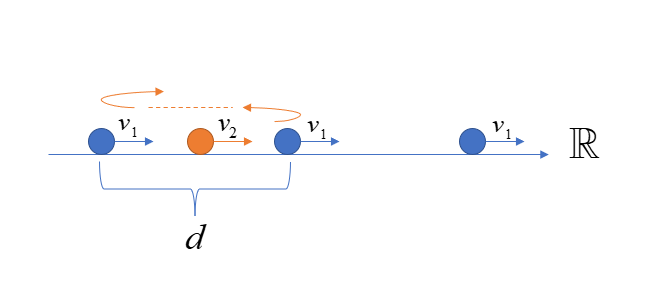
\includegraphics[scale=0.5]{на прямой.png}\\
\end{center}

На данном рисунке лидеры отмечены синим цветом, а участники оранжевым. В условиях данной модели (пока еще детерминированной), можно ввести скорости сближения лидера и участника $u_{-} = v_2 + v_1$ ("\,-"\, здесь отображает направление скорости участника относительно вещественной оси), и скорость отдаления \\
$u_{+} = v_2 - v_1$. Пусть положение участника на оси и его скорость описываются процессами $x_2(t)$ и $v_2(t)$ соответственно. Аналогичным образом определим $x_1(t)$ и $v_1(t)$ как процессы, описывающие координату лидера и его скорость. В новых обозначениях построим график расстояния между участником и предшествующим ему лидером в зависимости от времени $y(t) = x_2 (t) - x_1(t)$. Он будет иметь следующий вид.
\begin{center}
    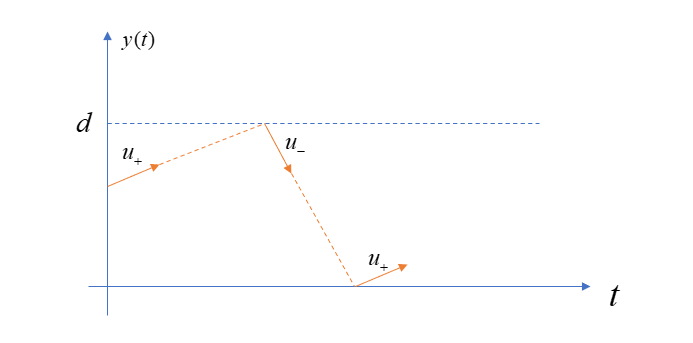
\includegraphics[scale=1]{детерм.png}\\
\end{center}

Попробуем теперь немного усложнить задачу и добавить "случайность"\,. Предположим, что в моменты скачков пуассоновского процесса $ \Pi_t (\alpha)$ с интенсивностью $\alpha$ мы разворачиваем скорость участника. В таком случае график выше может принимать другие формы.
\begin{center}
    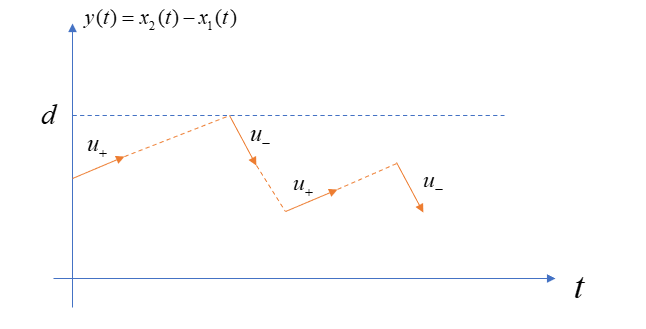
\includegraphics[scale=0.5]{стохаст.png}\\
\end{center}

Рассмотрим далее двумерный стохастический процесс 
\begin{equation*}
\xi_t = \begin{pmatrix}
 y(t) \\
 v(t)
\end{pmatrix}, \qquad 
\begin{aligned}
y(t) &= x_2(t) - x_1(t) \in \mathbb{R} \\
v(t) &= v_2(t) - v_1(t) \in \left\{ u_+, u_- \right\} 
\end{aligned}
\end{equation*}
Мы хотим установить, существует ли стационарное распределение процесса $\xi_t$, и если да, то найти его явный вид.

\section{Стационарное распределение процесса $\xi_t$}\label{section_2}

Рассмотрим оператор $P^t$ в пространстве $\textbf{B}$ ограниченных функций такой, что для $f \in \textbf{B}$
\begin{equation}\label{1}
P^t f(x) = \int f(z) P(x, t, dz),
\end{equation}
где $P (x, t, \Gamma)$ - переходная функция марковского процесса $\xi_t$. С другой стороны, выражение ~\eqref{1} можно представить в виде 
$$P^t f (x) = E \left( f (\xi_t) | \xi_0 = x \right) =: \mathbf{E}_x f (\xi_t).$$
В пространстве счетно-аддитивных функций множеств $\textbf{V}$ оператор $P^t$ можно определить на $\nu \in \textbf{V}$, как
\begin{equation*}
\nu P^t (\Gamma) = \int\displaylimits_X \nu (dx) P(x, t, \Gamma).
\end{equation*}

Инфинитезимальный оператора $A$ определен на элементе $f \in \textbf{B}$ и равен
\begin{equation}\label{infinit}
    A f(x) = \lim_{t \downarrow 0} t^{-1} \left( P^t f(x) - f(x) \right),
\end{equation}
если этот предел по норме существует. Поскольку мы рассматриваем функции $f \in \textbf{B}$ из пространства ограниченных функций с нормой
\begin{equation}\label{norma}
    \left\| f \right\| = \underset{x \in X}{\sup} |f(x)|,
\end{equation}
то \ref{infinit} можно переписать в виде
$$A f(x) = \lim_{t \downarrow 0} t^{-1} \left( P^t f(x) - f(x) \right) = \lim_{t \downarrow 0} t^{-1} \left( \mathbf{E}_x f (\xi_t) - f(x) \right),$$
причем $f \in D_A$, если этот предел равномерен по $x$. Для полугруппы $P^t$, действующей на меры, мы также можем рассматривать инфинитезимальный оператор $A$ на $\mu \in \textbf{V}$
$$\mu A = \lim_{t \downarrow 0} t^{-1} \left( \mu P^t - \mu \right)$$
в смысле сходимости по вариации.
Тогда имеет место следующее соотношение $\left\langle \mu, A f \right\rangle = \left\langle \mu A, f\right\rangle$. 

Инфинитезимальный оператор $A$ представляет собой характеристику, которая задает полугруппу операторов $P^t$ с точностью до малых выше первого порядка. Она также однозначно определяет переходную функцию.


Важным приложением этой теории является нахождение стационарного распределения по инфинитезимальному оператору. Стационарным распределением называют вероятностную инвариантную меру, т. е. меру $\mu$ такую, что выполнено условие $\mu \equiv \mu P^t, \, t \geq 0$ и $\mu (X) = 1$. 
Из $\mu P^t \equiv \mu$ следует, что $\mu A = 0$, и дело сводится к тому, чтобы найти ненулевое неотрицательное решение уравнения $\mu A = 0$ и пронормировать его, разделив на $\mu (X)$.

В условиях нашей модели, мы будем считать, что функции $f ( x )$ отображают множество $X = X_+ \bigsqcup X_-$ в $\mathbb{R}$, где $X_+ = [0, d) \times \left\{u_+\right\}$ и $X_- = (0, d] \times \left\{u_-\right\}$. Таким образом, мы будем работать с функциями $f_- (y): X_- \to \mathbb{R}$ и $f_+ (y): X_+ \to \mathbb{R}$ такими, что
$$
f(x) = \left\{ \begin{array}{cl}
f_+ ( y ) & , \ x = \left( y, u_+ \right) \\
f_- ( y ) & , \ x = \left( y, u_- \right) 
\end{array} \right.
$$
После того как все необходимые обозначения введены, сформулируем и докажем следующее утверждение.
\begin{utv}
Инфинитезимальный оператор полугруппы $P^h f$, связанной с процессом $\xi_t$, действует на $f(x): X \to \mathbb{R}$ следующим образом
\begin{equation}
A f(x) =
\left\{ \begin{aligned} 
  -u_- f_-' (y) - \alpha f_- (y) + \alpha f_+ (y), \qquad x &= (y, u_-),  \quad  y \in (0, d)\\
  u_+ f_+' (y) - \alpha f_+ (y) + \alpha f_- (y), \qquad  x &= (y, u_+),  \quad  y \in (0, d)\\
  \frac{\alpha u_-}{u_- + u_+} (f_+ (d -  0) - f_- (d)) - u_- f_-' (d), \qquad  x &= (d, u_-)\\
  \frac{\alpha u_+}{u_- + u_+} (f_- (0 + 0) - f_+ (0)) + u_+ f_+' (0), \qquad  x &= (0, u_+)
\end{aligned} \right.
\end{equation}
 Здесь $f_- (y) \in \mathrm{C}^{(1)} (0, d]$, $f_+ (y) \in \mathrm{C}^{(1)} [0, d)$ и существуют конечные пределы $f_- (0 + 0)$ и $f_+ (d -  0)$ на границах $y = 0$ и $y = d$ (на границах также подразумевается наличие односторонних производных).
\end{utv}
{\bf Доказательство}\\
Зафиксируем начальное положение $x = \begin{pmatrix}
 y \\
 u_-
\end{pmatrix} $, где $y \in (0, d)$, и вычислим согласно ~\eqref{1} чему равно $P^h f (x) $ за малый промежуток времени $h$.
Имеем,
$$P^h f  \begin{pmatrix}
 y \\
 u_-
\end{pmatrix}  = f_- (y - h u_-) P (N_h = 0) + f_+ (y_h) P(N_h = 1) + o (h) =$$
$$ = f_- (y - h u_-) e^{- \alpha h} + f_+ (y_h) e^{- \alpha h} \alpha h + o(h).$$
Здесь $N_t$ есть число перемен знака скорости за время $t$, т. е. случайная величина, имеющая распределение Пуассона с параметром $\alpha t$, а $y_h$ есть некоторая точка из интервала $(y - h u_-, y + h u_+)$.

Далее,
$$\frac{P^h f (x) - f(x)}{h} = \frac{f_- (y - h u_-) e^{-\alpha h} - f_- (y)}{h} + f_+ (y_h) e^{- \alpha h} \alpha + o (1)$$
Прибавим и вычтем в числителе первого слагаемого значение $f_- (y) e^{- \alpha h}$, тогда слагаемое представимо в следующем виде
\begin{equation*}
    \begin{aligned}
   \frac{f_- (y - h u_-) e^{-\alpha h} - f_- (y)}{h} &= u_- e^{- \alpha h} \frac{f_- (y - h u_-) - f_- (y)}{h u_-}
    &+ f_- (y) \frac{e^{- \alpha h} - 1}{h}
    \end{aligned}
\end{equation*}
Пользуясь определением дифференцируемости в точке $y \in (0, d)$, разложением экспоненты в ряд Тейлора в нуле и непрерывностью функции $f_+ (y_h)$ при $y_h \to y$, имеем
$$ A f(x) = \lim_{h \downarrow 0} \frac{\left( P^h f(x) - f(x) \right)}{h} = -u_- f_-' (y) - \alpha f_- (y) + \alpha f_+ (y).$$
Аналогичным образом найдем действие оператора для $x = \begin{pmatrix}
 y \\
 u_+
\end{pmatrix}:$
\begin{equation*}
    \begin{aligned}
  &\lim_{h \downarrow 0} \frac{ f_+ (y + h u_+) P (N_h = 0) + f_- (y_h) P(N_h = 1) - f_+(y) }{h} + o(1) = \\
 = &\lim_{h \downarrow 0} \frac{f_+ (y + h u_+) e^{-\alpha h} - f_+ (y)}{h} + f_- (y_h) e^{- \alpha h} \alpha  = \\
= &\lim_{h \downarrow 0} u_+ e^{- \alpha h} \frac{f_+ (y + h u_+) - f_+ (y)}{h u_+} + f_+ (y) \frac{e^{- \alpha h} - 1}{h} + f_- (y_h) e^{- \alpha h} \alpha = \\
 = &u_+ f_+' (y) - \alpha f_+ (y) + \alpha f_- (y) = A f (x).
    \end{aligned}
\end{equation*}

Рассмотрим отдельно поведение в пределах границ.
Прежде всего обратим внимание на то, что точки $x^0_+ = 
\begin{pmatrix}
 0 \\
 u_+
\end{pmatrix}$ и $x^0_- = 
\begin{pmatrix}
 0 \\
 u_-
\end{pmatrix}$, а также $x^d_+ = 
\begin{pmatrix}
 d \\
 u_+
\end{pmatrix}$ и $x^d_- = 
\begin{pmatrix}
 d \\
 u_-
\end{pmatrix}
$ можно отождествить. Действительно, поведение частицы на границах детерминировано и не зависит от скорости, с которой эта частица налетает на границу. Таким образом, без ограничения общности будем считать, что в граничных точках $y = 0$ и $y = d$ скорость принимает новое значение, т. е. $u_+$ и $u_-$ соответственно. Обозначим за $N_{[a, b]}$ число переключений скоростей на отрезке времени $[a, b]$. Итак, рассмотрим действие оператора ~\eqref{1} на $f \begin{pmatrix}
 d \\
 u_-
\end{pmatrix}$. Имеем,
\begin{equation*}
    \begin{aligned}
  P^h f \begin{pmatrix}
 d \\
 u_-
\end{pmatrix} &= f_- (d - h u_-) P (N_{[0, h]} = 0) + f_-(y^h_-) P (N_{[0, t_-]} = 1, N_{[t_-, h]} = 0) +\\
&+ f_+(y^h_+) P (N_{[0, t_-]} = 0, N_{[t_-, h]} = 1) + o(h).      
    \end{aligned}
\end{equation*}
Здесь $t_- = \displaystyle\frac{h u_+}{u_- + u_+}$ - это время, в течение которого частица, двигающаяся со скоростью $u_-$, окажется на таком расстоянии от границы $y = d$, что за оставшееся время $h - t_-$ его с точностью можно преодолеть со скоростью $u_+$. Подробнее,
\begin{equation*}
\begin{aligned}
\left\{\begin{matrix}
 t_+ u_+ - t_- u_- &= 0 \\
 t_+ + t_- &= h
\end{matrix}
\right. \qquad
&\Rightarrow \Bigl( h - t_-\Bigr) u_+ - t_- u_- = 0\\
&\Rightarrow t_- := \frac{h u_+}{u_- + u_+} \Rightarrow t_+ : = h - t_- = \frac{h u_-}{u_- + u_+}.
\end{aligned}
\end{equation*}
 Иначе говоря, если частица со скоростью $u_-$ поменяет ее на отрезке времени $[0, t_-]$, то она еще раз отразится от границы.
В силу независимости случайных величин $N_{[a, b]} \sim \text{Pois} (\alpha \cdot (b - a))$ с непересекающимися отрезками, имеем
\begin{equation*}
    \begin{aligned}
  P (N_{[0, t_-]} = 1, N_{[t_-, h]} = 0) &= P (N_{[0, t_-]} = 1) \cdot P (N_{[t_-, h]} = 0) = \\
 &= \alpha t_- e^{-\alpha t_-} \cdot e^{-\alpha (h - t_-)} = \alpha t_- e^{- \alpha h},\\
 P (N_{[0, t_-]} = 0, N_{[t_-, h]} = 1) &= P (N_{[0, t_-]} = 0) \cdot P (N_{[t_-, h]} = 1) = \\
&= e^{- \alpha t_-} \cdot \alpha (h - t_-) e^{- \alpha (h - t_-)} = \alpha (h - t_-) e^{- \alpha h}
    \end{aligned}
\end{equation*}
С учетом обозначений $t_+ = h - t_-$ получим
$$P^h f \begin{pmatrix}
 d \\
 u_-
\end{pmatrix} = f_- (d - h u_-) e^{- \alpha h} + f_- (y^h_-) \alpha t_- e^{- \alpha h} + f_+ (y^h_+ ) \alpha t_+ e^{- \alpha h} + o(h)$$
Найдем теперь инфинитезимальный оператор. Для этого рассмотрим следующее выражение при $x^d_- = 
\begin{pmatrix}
 d \\
 u_-
\end{pmatrix}
$:
\begin{equation*}
    \begin{aligned}
  \frac{P^h f (x^d_-) - f (x^d_-)}{h} &= u_- e^{- \alpha h} \frac{f_- (d - h u_-) - f_- (d)}{h u_-} + f_- (d) \frac{e^{- \alpha h} - 1}{h} + \\
&+ f_- (y^h_-) \alpha \frac{t_-}{h} e^{- \alpha h} + f_+ (y^h_+ ) \alpha \frac{t_+}{h} e^{- \alpha h} + o(1). 
    \end{aligned}
\end{equation*}
После того, как перейдем к пределу по $h \to 0$, получим
\begin{equation*}
    \begin{aligned}
  A f \begin{pmatrix}
 d \\
 u_-
\end{pmatrix} &= - u_- f_-' (d) - \alpha f_- (d) + \frac{\alpha}{u_- + u_+} \left(f_- (d) u_+ + f_+ (d - 0) u_- \right) =\\
&= \frac{\alpha u_-}{u_- + u_+} (f_+ (d - 0) - f_- (d)) - u_- f_-' (d).      
    \end{aligned}
\end{equation*}
С помощью аналогичных рассуждения для $x_+^0 = \begin{pmatrix}
 0 \\
 u_+
\end{pmatrix}$ мы имеем
$$A f \begin{pmatrix}
 0 \\
 u_+
\end{pmatrix} = \frac{\alpha u_+}{u_- + u_+} (f_- (0 + 0) - f_+ (0)) + u_+ f_+' (0).$$
\begin{flushright}
$\blacksquare$
\end{flushright}

\begin{zam}
Как уже было сказано ранее, все вышестоящие пределы понимаются в смысле сходимости по норме ~\eqref{norma} и $f \in D_A$, если эти пределы равномерны по $x$. Тогда имеет место склейка в граничных точках. А именно, устремляя\\ $(y, u_-) \to (d, u_-)$ и
$(y, u_+) \to (0, u_+)$, справедливы следующие ограничения
\begin{equation*}
\begin{aligned} 
  -u_- f_-' (d) - \alpha f_- (d) + \alpha f_+ (d - 0) &= \frac{\alpha u_-}{u_- + u_+} (f_+ (d - 0) - f_- (d)) - u_- f_-' (d)\\
  u_+ f_+' (0) - \alpha f_+ (0) + \alpha f_- (0 + 0) &= \frac{\alpha u_+}{u_- + u_+} (f_- (0 + 0) - f_+ (0)) + u_+ f_+' (0).
\end{aligned}
\end{equation*}
Откуда вытекает, что
\begin{equation}\label{restrict}
\begin{aligned} 
  f_+ (d - 0) &= f_-(d)\\
  f_- (0 + 0) &= f_+(0)
\end{aligned}
\end{equation}
\end{zam}
Итак, с учетом замечаний и утверждений, приведенных выше, перейдем к доказательству теоремы.
\begin{theorem}
Существует инвариантная мера $\mu (\cdot)$ такая, что ее ограничения $\mu_+(\cdot)$ и $\mu_- (\cdot)$ на подмножества $X_+ = [0, d) \times \left\{u_+\right\}$ и $X_- = (0, d] \times \left\{u_-\right\}$ соответственно удовлетворяют следующим соотношениям:
\begin{enumerate}
\item $\mu_+ \{0\} = 0$
\item $\mu_- \{d\} = 0$
\item Mеры $\mu_\pm (\cdot)$ имеют плотности $g_\pm (y)$ при $y \in (0, d)$ такие, что
\begin{equation*}
    \begin{aligned}
        g_+ (y) &= \frac{C}{u_+} \cdot \rho (y), \quad x = ( y, u_+) \in X,\\
g_-(y) &= \frac{C}{u_-} \cdot \rho (y), \quad x = ( y, u_- ) \in X.
    \end{aligned}
\end{equation*}
Здесь 
$$\rho (y) : = \frac{- \beta e^{\beta y}}{1 - e^{\beta d}}, \quad y \in (0, d),$$
где $\beta = \alpha \left( \displaystyle\frac{u_+ - u_-}{u_+ u_-}\right) < 0$ и $C = \displaystyle\frac{u_+ u_-}{u_+ + u_-}.$

\end{enumerate}
\end{theorem}
{\bf Доказательство}

Мы хотим найти такую меру $\mu$ на множестве $X$, что $\left< \mu, A f\right> = 0$ для всех $f$ из области определения $A, D_A$. По определению $f \in D_A$, если рассматриваемые выше пределы равномерны по $x$. Таким образом, будем считать, что функция $f$ ограничена и равномерно непрерывна вместе с первой производной (на границах $y = 0$ и $y = d$ подразумевается наличие производной справа и слева соответственно), откуда \\$f_+ \in C^{(1)} [0, d)$ и $f_- \in C^{(1)} (0, d]$. 

Итак, имеет место следующее равенство,
\begin{equation}\label{2}
\begin{aligned}
&\int_0^d \Bigl( \alpha f_- (y) - \alpha f_+ (y) + u_+ f_+' (y) \Bigr) \mu_+ (dy) & + \\
 &+ \int_0^d \Bigl( \alpha f_+ (y) - \alpha f_- (y) - u_- f_-' (y) \Bigr) \mu_- (dy) & + \\
 &+ \mu_+ \{0\} \cdot u_+ f_+' (0) + \mu_- \{d\} \cdot \Bigl( - u_- f_-' (d)\Bigr)  & = 0 ,
\end{aligned}
\end{equation}
где $\mu_+(\cdot)$ и $\mu_- (\cdot)$ есть ограничения меры $\mu$ на подмножества $X_+ = [0, d) \times \{u_+\}$ и \\$X_- = (0, d] \times \{u_-\}$ соответственно. Будем искать такую меру $\mu (\cdot)$, чтобы ее ограничения на подмножества $X_+$ и $X_-$ можно было задать с помощью функций плотности
$$g_+ (y) := \frac{\mu_+ (dy)}{dy}, \quad g_- (y) := \frac{\mu_- (dy)}{dy}.$$

Следующие соображения очень схожи с теми, что представлены в книге А. Д. Вентцеля "Курс теории случайных процессов" \cite{Venz}.
Предположим, что 
$$f_+ (y) = f_- (y) = \displaystyle\int_0^y \psi (x) dx, \qquad y \in [0, d]$$
где $\psi (x) \in \mathrm{C}_{0} [0, d]$ и $\psi (0) = f_+' (0) =  \psi (d) = f_-' (d) = 0$. Заметим, что заданные таким образом функции удовлетворяют условиям на границах \eqref{restrict}. Тогда ~\eqref{2} примет вид
$$ \int_0^d u_+ \psi (y) \mu_+ (dy) = \int_0^d u_- \psi (y) \mu_- (dy).$$
Откуда в силу свойств интеграла Лебега и произвольности $\psi (\cdot)$ из класса $\mathrm{C}_0$ имеет место следующее соотношение на меры во внутренних точках $(0, d)$:
\begin{align}\label{3}
u_+ \mu_+ (dy) = u_- \mu_- (dy)
\end{align}

Предположим теперь, что $\psi (0) = f_+' (0) = 1, \psi (d) = f_-' (d) = 0$, откуда с учетом соотношения \eqref{3} имеем
$$\mu_+ \{0\} \cdot u_+ \cdot \psi (0) = 0 \Rightarrow \mu_+ \{0\} = 0.$$

Аналогично, при  $\psi (0) = f_+' (0) = 0, \psi (d) = f_-' (d) = 1$ получаем
$$\mu_- \{d\} \cdot u_- \cdot \psi (d) = 0 \Rightarrow \mu_- \{d\} = 0.$$
Заметим, что в терминах плотностей соотношение ~\eqref{3} эквивалентно
\begin{equation}\label{density_eq}
    u_+ g_+(y) = u_- g_- (y), \quad y \in (0, d).
\end{equation}

Представим теперь, что $f_- (y) \equiv 0$ на $[0, d]$ и $f_+ (y) = f(y) \in C^{(1)} [0, d].$ Причем в силу ограничений \eqref{restrict} на границах должны выполняться следующие условия
\begin{equation}\label{bord_cond}
    f (0) = 0, \quad f(d) = 0.
\end{equation}
Тогда, соотношение \eqref{2} есть
\begin{equation*}
    \begin{aligned}
    &\int_0^d \Bigl( u_+ f' (y) - \alpha f (y) \Bigr) g_+(y) dy + \int_0^d \Bigl( \alpha f (y) \Bigr) g_- (y) dy = 0 \\
   \implies &- \int_0^d u_+ f' (y) g_+(y) dy = \int_0^d \alpha f (y) \Bigl( g_- (y) - g_+ (y)\Bigr) dy
    \end{aligned}
\end{equation*}
Пользуясь формулой интегрирования по частям, а также граничными условиями ~\eqref{bord_cond}, получим
\begin{equation*}
    \begin{aligned}
    &- u_+ f (y) g_+(y) \Bigl|_0^d + \int_0^d u_+ f (y) g_+'(y) dy = \int_0^d \alpha f (y) \Bigl( g_- (y) - g_+ (y)\Bigr) dy\\
    \implies & \int_0^d u_+ f (y) g_+'(y) dy = \int_0^d \alpha f (y) \Bigl( g_- (y) - g_+ (y)\Bigr) dy.
    \end{aligned}
\end{equation*}
Аналогичным образом, в силу произвольности $f (y) \in C^{(1)} [0, d]$, имеем
\begin{equation}\label{dif_eq_+}
    g_+' (y) = \frac{\alpha}{u_+} \cdot \Bigl( g_- (y) - g_+ (y) \Bigr), \quad y \in (0, d).
\end{equation}
Введем следующее обозначение $\beta := \alpha \cdot \left( \displaystyle\frac{u_+ - u_-}{u_+ u_-}\right) < 0$. Тогда, выражая $g_- (y)$ через $g_+ (y)$ согласно ~\eqref{density_eq}, получим 
$$ g_+' (y) = \beta g_+(y) $$
Решая данное дифференциальное уравнение, находим явный вид $g_+(y)$ с точностью до константы $\widetilde{C}$
\begin{equation*}
    \begin{aligned}
        &\int \frac{g_+' (y)}{g_+ (y)} dy = \int \beta dy\\
        \implies &\ln g_+(y) = \beta y + \widetilde{C}\\
        \implies &g_+ (y) = \widetilde{C} \cdot e^{\beta y}, \quad y \in (0, d)
    \end{aligned}
\end{equation*}
Из соотношения на плотности ~\eqref{density_eq} следует
$$g_- (y) = \frac{u_+}{u_-} g_+ (y), \quad y \in (0, d).$$
Учитывая последнее равенство, найдем нормирующую константу $\widetilde{C}$ из условия
\begin{equation*}
    \begin{aligned}
   \mu (X) := \mu_+ ([0, d)) + \mu_- ((0, d]) &= 1\\
\implies \widetilde{C} \left( 1 + \frac{u_+}{u_-} \right) \int_0^d e^{\beta x} dx &= 1     
    \end{aligned}
\end{equation*}
 Тогда
\begin{equation*}
    \begin{aligned}
   \frac{\widetilde{C}}{\beta} \left( 1 + \displaystyle\frac{u_+}{u_-}\right) \left[ e^{\beta d} - 1\right] &= 1\\
\implies \widetilde{C} = \frac{- \beta u_-}{(u_+ + u_-) [1 - e^{\beta d}]} &> 0     
    \end{aligned}
\end{equation*}
Таким образом, если ввести обозначение 
$$\rho (y) : = \frac{- \beta e^{\beta y}}{1 - e^{\beta d}},$$
то итоговые плотности примут следующий вид
\begin{equation*}
    \begin{aligned}
  g_+ (y) &= \frac{u_-}{u_+ + u_-} \cdot \rho (y), \quad y \in (0, d)\\
g_- (y) &= \frac{u_+}{u_-} g_+ (y) = \frac{u_+}{u_+ + u_-} \cdot \rho (y), \quad y \in (0, d). 
    \end{aligned}
\end{equation*}
Откуда, определив константу $C = \displaystyle \frac{u_+ u_-}{u_+ + u_-}$, имеем
\begin{equation*}
    \begin{aligned}
        g_+ (y) &= \frac{C}{u_+} \cdot \rho (y), \quad y \in (0, d)\\
g_-(y) &= \frac{C}{u_-} \cdot \rho (y), \quad y \in (0, d).
    \end{aligned}
\end{equation*}

\begin{flushright}
$\blacksquare$
\end{flushright}

\begin{zam}
Рассмотрим функции $f_+ (y) \equiv 0$ на $[0, d]$ и $f_- (y) = f (y) \in C^{(1)} [0, d]$, где $f$ удовлетворяет граничным условиям ~\eqref{bord_cond}. Проделав аналогичные рассуждения для выражения ~\eqref{2} с заданными функциями, приходим к следующему дифференциальному уравнению
\begin{equation*}
    g_-' (y) = \frac{\alpha}{u_-} \cdot \Bigl( g_- (y) - g_+ (y) \Bigr), \quad y \in (0, d).
\end{equation*}
Тогда, с учетом ~\eqref{dif_eq_+} имеет место система дифференциальных уравнений
\begin{equation}\label{simple_case}
    \begin{aligned}
        \left\{\begin{matrix}
            g_+' (y) = \displaystyle\frac{\alpha}{u_+} \cdot \Bigl( g_- (y) - g_+ (y) \Bigr), \quad y \in (0, d)\\
            g_-' (y) = \displaystyle\frac{\alpha}{u_-} \cdot \Bigl( g_- (y) - g_+ (y) \Bigr), \quad y \in (0, d)
        \end{matrix}\right.
    \end{aligned}
\end{equation}
\end{zam}

Итак, мы нашли стационарное распределение, то есть такое распределение процесса $\xi_t$, что оно не меняется с течением времени. 

\begin{sled}
Стационарное распределение скорости $v(t)$ при $t \ge 0$ удовлетворяет
\begin{equation*}
\begin{aligned}
    P (v(t) = u_+) = \frac{u_-}{u_+ + u_-},\\
    P (v(t) = u_-) = \frac{u_+}{u_+ + u_-}.
    \end{aligned}
\end{equation*}
\end{sled}
{\bf Доказательство}\\
Поскольку мы уже знаем совместное стационарное распределение $\xi_t = \begin{pmatrix}
 y(t) \\
 v(t)
\end{pmatrix}$, то стационарное распределение компоненты $v(t)$ удовлетворяет
\begin{equation*}
    \begin{aligned}
        P (v(t) = u_+) = \int_0^d g_+(y) dy = \frac{u_-}{u_+ + u_-}, \quad t \ge 0\\
        P (v(t) = u_-) = \int_0^d g_-(y) dy = \frac{u_+}{u_+ + u_-}, \quad t \ge 0
    \end{aligned}
\end{equation*}
\begin{flushright}
$\blacksquare$
\end{flushright}

\section{Общие свойства стационарной плотности}
Мы получили стационарные плотности следующего вида 
\begin{equation*}
    \begin{aligned}
        g_+ (y) &= \frac{C}{u_+} \cdot \rho (y), \quad y \in (0, d)\\
g_-(y) &= \frac{C}{u_-} \cdot \rho (y), \quad y \in (0, d).
    \end{aligned}
\end{equation*}
где
$$\rho (y) : = \frac{- \beta e^{\beta y}}{1 - e^{\beta d}}, \qquad C = \displaystyle \frac{u_+ u_-}{u_+ + u_-} > 0, \quad \beta = \alpha \cdot \left( \displaystyle\frac{u_+ - u_-}{u_+ u_-}\right) < 0.$$

В силу неравенства $u_+ < u_-$ для каждого $y \in (0, d)$ имеем $g_- (y) < g_+ (y)$ и графики плотностей имеют следующий вид
\begin{center}
\begin{tikzpicture}[domain=0:5]
\draw[very thin,color=gray] (-0.1,-0.1) grid (5.5,4.5);
\draw[->] (-0.2,0) -- (6,0) node[right] {$x$};
\draw[->] (0,-0.2) -- (0,5) node[above];
\draw[color=red] plot (\x,{2*exp(-\x/2.5)}) node[right] {$g_-(x)$};
\draw[color=blue] plot (\x,{4*exp(-\x/2.5)}) node[above] {$g_+ (x)$};
\draw (-0.2cm,2pt) node[below] {$0$};
\draw (5cm,2pt) node[below] {$d$};

\end{tikzpicture}
\end{center}

Тот факт, что плотности убывают на $(0, d)$ и достигают своего максимума в точке $0$, можно объяснить тем, что на большом отрезке времени суммарный сдвиг траектории убывает. Действительно, обозначим за $\left\{t_i, i = 1,2...\right\}$ моменты переключения скоростей движущейся частицы. Величины $T_i := t_i - t_{i - 1}$, описывающие длительность пребывания процесса в данном состоянии, являются независимыми с распределением $\text{Exp} (\alpha)$ \cite{Karl}. В силу того, что $u_- > u_+$, смещение траектории вниз за "равные" (равнораспределенные) отрезки времени будет преобладать.
\begin{center}
    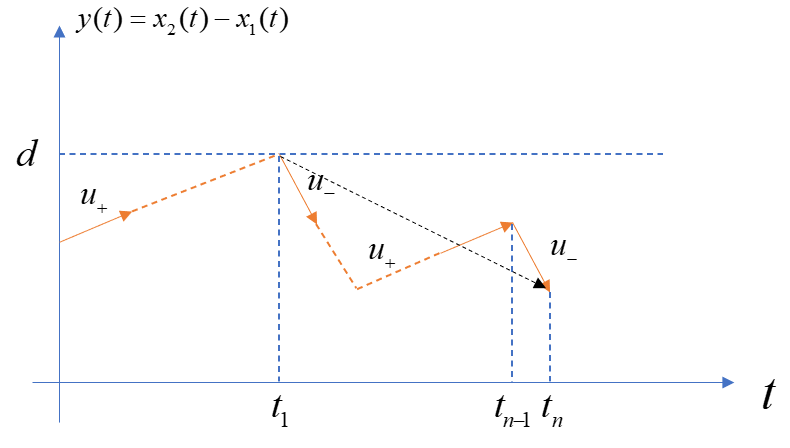
\includegraphics[scale=0.4]{итог_сдвиг.png}\\
\end{center}
Далее заметим, что большим значениям параметра интенсивности $\alpha$ соответствует больший наклон графиков. Таким образом, мера сосредоточена вблизи нижней границы, что, с учетом замечания о суммарном сдвиге, весьма естественно, ведь чем больше колеблется частица, тем меньше вероятность ее выхода на верхнюю границу. И напротив, если параметр $\alpha$ мал, или значения $u_+$ близки к $u-_$, то $\beta$ близко к нулю и графики будут более пологими, близкими к константам. Иначе говоря, мера будет распределена более равномерно на интервале $(0, d).$
\section{Модель с возмущением верхней границы}

Представим теперь, что верхняя граница компонентны $y(t)$ подвержена возмущениям. А именно, пусть положение границы задается следующим марковским процессом
\begin{equation*}
    r(t) = r_t = (-1)^{\Pi_t(\gamma)} \cdot \frac{L}{2} + \Bigl( d + \frac{L}{2}\Bigr),
\end{equation*}
где $\Pi_t (\gamma)$ - есть пуассоновский процесс с интенсивностью $\gamma$. Таким образом, $r_t$ принимает значения в множестве $\left\{ d, d + L\right\}$. Более того, будем считать, что процессы $r_t$ и $\xi_t$ независимы. 

При заданной постановке задачи возникает вопрос, что происходит с частицей, находящейся в зоне $y(t) > d$, в момент времени, когда граница опускается до уровня $d$? Мы будем считать, что в таком случае частица совершает скачок в точку \\$(d, u_-) \in X$.
\begin{center}
    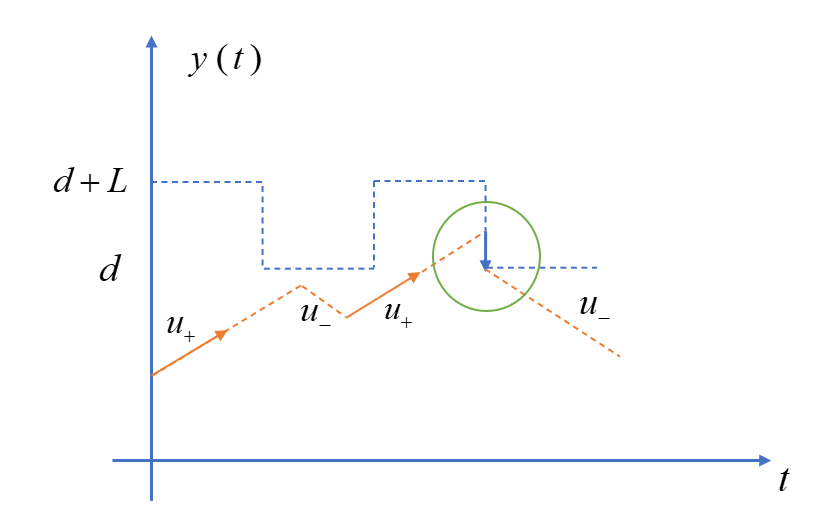
\includegraphics[scale=0.4]{new_model.png}\\
\end{center}

Далее будем рассматривать трехмерный стохастический процесс
\begin{equation*}
\begin{aligned}
\eta_t &= \Bigl( y(t), v(t), r(t)\Bigr)^\intercal, \\
y(t) &= x_2(t) - x_1(t) \in \mathbb{R}, \\
v(t) &= v_2(t) - v_1(t) \in \left\{ u_+, u_- \right\}, \\
r(t) &\in \left\{d, d + L\right\}.
\end{aligned}
\end{equation*}

Итак, в условиях новой задачи попробуем установить, существует ли стационарное распределение процесса $\eta_t$ и по возможности исследуем его характеристики.

Воспользуемся уже изложенной выше теорией и будем рассматривать функции $f: Z \to \mathbb{R}$, где 
\begin{equation*}
Z = Z_{0, +}\bigsqcup Z_{1, +}\bigsqcup Z_{0, -}\bigsqcup Z_{1, -}
\end{equation*}
и \\
$Z_{0, +} = [0, d) \times \{u_+\} \times \{d\} $, 
\\
$Z_{1, +} = [0, d + L) \times \{u_+\} \times \{d + L\} $,
\\ $Z_{0, -} = (0, d] \times \{u_-\} \times \{d\} $, 
\\
$Z_{1, -} = (0, d + L] \times \{u_-\} \times \{d + L\}$.\\
Далее,
\begin{equation*}
f(z) = \left\{ \begin{array}{cl}
f_{0, +} ( y ) , \quad z &= \left( y, u_+, d \right), \quad  y \in [0, d)\\
f_{0, -} ( y ) , \quad z &= \left( y, u_-, d \right), \quad  y \in (0, d] \\
f_{1, +} ( y ) , \quad z &= \left( y, u_+, d + L \right), \quad  y \in [0, d + L) \\
f_{1, -} ( y ) , \quad z &= \left( y, u_-, d + L \right), \quad  y \in (0, d + L] 
\end{array} \right.
\end{equation*}
В дальнейшем, для удобства записи, если какое-то свойство имеет силу \textit{для каждой вышестоящей функции}, определенной на своем полуинтервале, то будем говорить, что это свойство имеет силу \textit{для $f_{\theta, \pm}$}. Так, например, $f_{\theta, \pm} (y) \in C^{(1)}$.
\begin{utv}\label{utv_2}
Инфинитезимальный оператор полугруппы $P^h f$, связанной с процессом $\eta_t$, действует на $f(z): Z \to \mathbb{R}$ следующим образом
\begin{equation*}
\null \hspace*{-3cm} A f(z) =
\left\{ \begin{aligned} 
   -u_- f_{0,-}' (y) + \alpha \Bigl(f_{0,+}(y) - f_{0,-}(y) \Bigr) + \gamma \Bigl(f_{1,-} (y) - f_{0,-} (y) \Bigr) , \quad z &= (y, u_-, d),  \quad  y \in (0, d)\\
   u_+ f_{0,+}' (y) - \alpha \Bigl(f_{0,+}(y) - f_{0,-}(y) \Bigr) + \gamma \Bigl(f_{1,+} (y) - f_{0,+} (y) \Bigr), \quad  z &= (y, u_+, d),  \quad  y \in (0, d)\\
   -u_- f_{1,-}' (y) + \alpha \Bigl(f_{1,+}(y) - f_{1,-}(y) \Bigr) + \gamma \Bigl(f_{0,-} (y) - f_{1,-} (y) \Bigr), \quad  z &= (y, u_-, d + L), \quad y \in (0, d]\\
   -u_- f_{1,-}' (y) + \alpha \Bigl(f_{1,+}(y) - f_{1,-}(y) \Bigr) + \gamma \Bigl(f_{0,-} (d) - f_{1,-} (y) \Bigr), \quad  z &= (y, u_-, d + L), \quad y \in (d, d + L)\\
   u_+ f_{1,+}' (y) - \alpha \Bigl(f_{1,+}(y) - f_{1,-}(y) \Bigr) + \gamma \Bigl(f_{0,+} (y) - f_{1,+} (y) \Bigr), \quad  z &= (y, u_+, d + L), \quad y \in (0, d)\\
   u_+ f_{1,+}' (y) - \alpha \Bigl(f_{1,+}(y) - f_{1,-}(y) \Bigr) + \gamma \Bigl(f_{0,-} (d) - f_{1,+} (y) \Bigr), \quad  z &= (y, u_+, d + L), \quad y \in [d, d + L)\\
   \frac{\alpha u_+}{u_- + u_+} \Bigl(f_{0,-} (0) - f_{0,+} (0)\Bigr) + \gamma \Bigl( f_{1,+} (0) - f_{0,+} (0) \Bigr) + u_+ f_{0,+}' (0), \quad z &= (0, u_+, d)\\
    \frac{\alpha u_+}{u_- + u_+} \Bigl(f_{1,-} (0) - f_{1,+} (0)\Bigr) + \gamma \Bigl( f_{0,+} (0) - f_{1,+} (0) \Bigr) + u_+ f_{1,+}' (0), \quad  z &= (0, u_+, d + L)\\
   \frac{\alpha u_-}{u_- + u_+} \Bigl(f_{0,+} (d) - f_{0,-} (d)\Bigr) + \gamma \Bigl( f_{1,-} (d) - f_{0,-} (d) \Bigr) - u_- f_{0,-}' (d), \quad  z &= (d, u_-, d)\\
   \frac{\alpha u_-}{u_- + u_+} \Bigl(f_{1,+} (d + L) - f_{1,-} (d + L)\Bigr) + \gamma \Bigl( f_{0,-} (d) - f_{1,-} (d + L) \Bigr) &- u_- f_{1,-}' (d + L), \\  z = (d + L, u_-, d + L)
\end{aligned} \right.
\end{equation*}
Здесь $f_{\theta, \pm} (y) \in C^{(1)}$ и на границах своих областей определения существуют конечные пределы $f_{\theta, \pm} ( \cdot )$, а также предполагается наличие односторонних производных.
\end{utv}
\textbf{Доказательство}

Итак, рассмотрим различные варианты начального положения $z$ частицы и за малый промежуток времени $h$ рассмотрим действие оператора $P^h f (z)$.\\
\\
1) Пусть начальное положение частицы задается как  $z = \left(y, u_-, d\right)^\intercal$, где $y \in (0, d)$.
Введём новую случайную величину $Z_h$ с распределением Пуассона с параметром интенсивности $\gamma h$, отвечающую за число переключений границы за время $h$. Тогда оператор $P^h f (z)$ при $z = \left(y, u_-, d\right)^\intercal$ можно записать в следующем виде
\begin{equation*}
    \begin{aligned} 
  P^h f (z) &= P (Z_h = 0) \Bigl[f_{0, -} (y - h u_-) P (N_h = 0) + f_{0, +} (y_h) P(N_h = 1) \Bigr]  + \\
  & + P (Z_h = 1) \left[f_{1, -} (y - h u_-) P (N_h = 0) + f_{1, +} (y_h) P(N_h = 1) \right] + o (h) =\\
  & = e^{- \gamma h} \Bigl[f_{0,-} (y - h u_-) e^{- \alpha h} + f_{0, +} (y_h) e^{- \alpha h} \alpha h \Bigr] +\\
  & + e^{- \gamma h} \gamma h \Bigl[f_{1,-} (y - h u_-) e^{- \alpha h} + f_{1, +} (y_h) e^{- \alpha h} \alpha h \Bigr] + o(h).
\end{aligned}
\end{equation*}
Здесь $y_h$ есть некоторая точка из интервала $(y - h u_-, y + h u_+)$.
Заметим, что слагаемое вида  $P(Z_h = 1) \cdot P(N_h = 1)$ является бесконечно малой величиной второго порядка малости, т. е. $o(h)$ при $h \to \infty$. Действительно,
$$P(Z_h = 1) \cdot P(N_h = 1) = e^{- (\gamma + \alpha) h} \cdot \gamma \alpha h^2 = o(h).$$
Далее,
\begin{equation*}
    \begin{aligned}
  \frac{P^h f (z) - f(z)}{h} &= \frac{f_{0,-} (y - h u_-) e^{-(\gamma + \alpha) h} - f_{0,-} (y)}{h} + \\
  & + \alpha f_{0,+} (y_h) e^{- (\gamma + \alpha) h} + \gamma f_{1,-} (y - h u_-) e^{- (\gamma + \alpha) h} + o (1)  
    \end{aligned}
\end{equation*}
Прибавим и вычтем в числителе первого слагаемого значение $f_{0,-} (y) e^{- (\gamma + \alpha) h}$, тогда получим
\begin{equation*}
    \begin{aligned}
        \frac{f_{0,-} (y - h u_-) e^{-(\gamma + \alpha) h} - f_{0,-} (y)}{h} &= u_- e^{- (\gamma + \alpha) h} \frac{f_{0,-} (y - h u_-) - f_{0,-} (y)}{h u_-} + \\
& + f_{0,-} (y) \frac{e^{- (\gamma + \alpha) h} - 1}{h}.
    \end{aligned}
\end{equation*}
Пользуясь определением дифференцируемости функции в точке $y \in (0, d)$, разложением экспоненты в ряд Тейлора в нуле и непрерывностью функции $f_{0,+} (y_h)$ при $y_h \to y$, для $z = \left(y, u_-, d\right)^\intercal$ имеем 
\begin{equation*}
    \begin{aligned}
   A f(z) = \lim_{h \downarrow 0} \frac{\left( P^h f(z) - f(z) \right)}{h} &= -u_- f_{0,-}' (y) - (\gamma + \alpha) f_{0,-}(y) + \alpha f_{0,+} (y) + \gamma f_{1,-} (y) = \\
   &= -u_- f_{0,-}' (y) + \alpha \Bigl(f_{0,+}(y) - f_{0,-}(y) \Bigr) + \gamma \Bigl(f_{1,-} (y) - f_{0,-} (y) \Bigr).
    \end{aligned}
\end{equation*}
2) Проделав аналогичные вычисления для $z = \left(y, u_+, d\right)^\intercal$, где $y \in (0, d)$, получим
\begin{equation*}
    \begin{aligned}
   A f(z) &= u_+ f_{0,+}' (y) - (\gamma + \alpha) f_{0,+} (y) + \alpha f_{0,-} (y) + \gamma f_{1,+} (y) = \\
   &= u_+ f_{0,+}' (y) - \alpha \Bigl(f_{0,+}(y) - f_{0,-}(y) \Bigr) + \gamma \Bigl(f_{1,+} (y) - f_{0,+} (y) \Bigr).
    \end{aligned}
\end{equation*}
3) Подробнее рассмотрим случай, когда начальное положение задается как \\
$z = \left(y, u_-, d + L\right)^\intercal$, где $y \in (0, d + L)$. Представим, что за время $h$ до скачка границы положение частицы удовлетворяет $y \leq d + h u_-$, тогда, если частица двигается с постоянной скоростью $u_-$, изменение границы никак не повлияет на её траекторию. В таком случае за время $h$ координата частицы будет принимать значение $y - h u_-$. В случае, когда $y > d + h u_-$ и скорость постоянна и равна $u_-$, частица претерпит скачок до уровня $d$ в силу того, что верхняя граница опустится до этого уровня. Таким образом, в силу малости $h$ можно рассматривать два случая, когда $y \in (0, d]$ и $y \in (d, d + L)$.

Итак, при $z = \left(y, u_-, d + L\right)^\intercal, \quad y \in (0, d]$ выражения принимают следующий вид
\begin{equation*}
    \begin{aligned} 
  P^h f (z) &= P (Z_h = 0) \Bigl[f_{1, -} (y - h u_-) P (N_h = 0) + f_{1, +} (y_h) P(N_h = 1) \Bigr]  + \\
  & + P (Z_h = 1) \cdot f_{0, -} (y - h u_-) P (N_h = 0) + o (h) =\\
  & = e^{- \gamma h} \Bigl[f_{1,-} (y - h u_-) e^{- \alpha h} + f_{1, +} (y_h) e^{- \alpha h} \alpha h \Bigr] +\\
  & + e^{- \gamma h} \gamma h \cdot f_{0,-} (y - h u_-) e^{- \alpha h} + o(h).
\end{aligned}
\end{equation*}
Откуда имеем
\begin{equation*}
    \begin{aligned}
   A f(z) &= -u_- f_{1,-}' (y) - (\gamma + \alpha) f_{1,-}(y) + \alpha f_{1,+} (y) + \gamma f_{0,-} (y) = \\
   &= -u_- f_{1,-}' (y) + \alpha \Bigl(f_{1,+}(y) - f_{1,-}(y) \Bigr) + \gamma \Bigl(f_{0,-} (y) - f_{1,-} (y) \Bigr).
    \end{aligned}
\end{equation*}
В случае же, когда $z = \left(y, u_-, d + L\right)^\intercal, \quad y \in (d, d + L)$, справедливо
\begin{equation*}
    \begin{aligned} 
  P^h f (z) &= P (Z_h = 0) \Bigl[f_{1, -} (y - h u_-) P (N_h = 0) + f_{1, +} (y_h) P(N_h = 1) \Bigr]  + \\
  & + P (Z_h = 1) \cdot f_{0, -} (y_d) P (N_h = 0) + o (h) =\\
  & = e^{- \gamma h} \Bigl[f_{1,-} (y - h u_-) e^{- \alpha h} + f_{1, +} (y_h) e^{- \alpha h} \alpha h \Bigr] +\\
  & + e^{- \gamma h} \gamma h \cdot f_{0,-} (y_d) e^{- \alpha h} + o(h).
\end{aligned}
\end{equation*}
Здесь, $y_d$ есть некоторая точка из $(d - h u_-, d]$. Таким образом, в силу непрерывности функций и $y_d \to d$ при $h \to 0$, получим
\begin{equation*}
    \begin{aligned}
   A f(z) &= -u_- f_{1,-}' (y) - (\gamma + \alpha) f_{1,-}(y) + \alpha f_{1,+} (y) + \gamma f_{0,-} (d) = \\
   &= -u_- f_{1,-}' (y) + \alpha \Bigl(f_{1,+}(y) - f_{1,-}(y) \Bigr) + \gamma \Bigl(f_{0,-} (d) - f_{1,-} (y) \Bigr).
    \end{aligned}
\end{equation*}
4) Аналогично, при $z = \left(y, u_+, d + L\right)^\intercal$, где $y \in (0, d + L)$, имеют место два случая.\\
При $y \in (0, d)$:
\begin{equation*}
    \begin{aligned} 
  P^h f (z) &= P (Z_h = 0) \Bigl[f_{1, +} (y + h u_+) P (N_h = 0) + f_{1, -} (y_h) P(N_h = 1) \Bigr]  + \\
  & + P (Z_h = 1) \cdot f_{0, +} (y + h u_+) P (N_h = 0) + o (h) =\\
  & = e^{- \gamma h} \Bigl[f_{1,+} (y + h u_+) e^{- \alpha h} + f_{1, -} (y_h) e^{- \alpha h} \alpha h \Bigr] +\\
  & + e^{- \gamma h} \gamma h \cdot f_{0,+} (y + h u_+) e^{- \alpha h} + o(h).
\end{aligned}
\end{equation*}
Откуда
\begin{equation*}
    \begin{aligned}
   A f(z) &= u_+ f_{1,+}' (y) - (\gamma + \alpha) f_{1,+}(y) + \alpha f_{1,-} (y) + \gamma f_{0,+} (y) = \\
   &= u_+ f_{1,+}' (y) - \alpha \Bigl(f_{1,+}(y) - f_{1,-}(y) \Bigr) + \gamma \Bigl(f_{0,+} (y) - f_{1,+} (y) \Bigr).
    \end{aligned}
\end{equation*}
И при $z = \left(y, u_+, d + L\right)^\intercal, \quad y \in [d, d+ L)$:
\begin{equation*}
    \begin{aligned} 
  P^h f (z) &= P (Z_h = 0) \Bigl[f_{1, +} (y + h u_+) P (N_h = 0) + f_{1, -} (y_h) P(N_h = 1) \Bigr]  + \\
  & + P (Z_h = 1) \cdot f_{0, -} (y_d) P (N_h = 0) + o (h) =\\
  & = e^{- \gamma h} \Bigl[f_{1,+} (y + h u_+) e^{- \alpha h} + f_{1, -} (y_h) e^{- \alpha h} \alpha h \Bigr] +\\
  & + e^{- \gamma h} \gamma h \cdot f_{0,-} (y_d) e^{- \alpha h} + o(h).
\end{aligned}
\end{equation*}
Выражение для инфинитезимального оператора примет вид
\begin{equation*}
    \begin{aligned}
   A f(z) &= u_+ f_{1,+}' (y) - (\gamma + \alpha) f_{1,+}(y) + \alpha f_{1,-} (y) + \gamma f_{0,-} (d) = \\
   &= u_+ f_{1,+}' (y) - \alpha \Bigl(f_{1,+}(y) - f_{1,-}(y) \Bigr) + \gamma \Bigl(f_{0,-} (d) - f_{1,+} (y) \Bigr).
    \end{aligned}
\end{equation*}
5) Нам остается рассмотреть случаи на границах отрезков $[0, d]$ или $[0, d + L]$. Для начала рассмотрим простой случай для $z = \left(0, u_+, d\right)^\intercal$ и $z = \left(0, u_+, d + L\right)^\intercal$. Интуитивно понятно, что изменения верхней границы отрезка не должны никак влиять на траектории частицы вблизи нижней границы. Прежде чем мы непосредственно в этом убедимся с помощью вычислений, вспомним, что в граничных случаях нами вводились промежуточные значения времени $t_- := \displaystyle\frac{h u_+}{u_- + u_+}$ и $t_+ := h - t_- = \displaystyle\frac{h u_-}{u_- + u_+}$ такие, что 
\begin{equation*}
    \begin{aligned}
  P (N_{[0, t_-]} = 1, N_{[t_-, h]} = 0) &= P (N_{[0, t_+]} = 0, N_{[t_+, h]} = 1) = \alpha t_- e^{- \alpha h},\\
  P (N_{[0, t_-]} = 0, N_{[t_-, h]} = 1) &= P (N_{[0, t_+]} = 1, N_{[t_+, h]} = 0) = \alpha t_+ e^{- \alpha h}.
    \end{aligned}
\end{equation*}
Взяв за основу уже проделанные вычисления в предыдущей секции ~\eqref{section_2}, выведем равенства для $z = \left(0, u_+, d\right)^\intercal$
\begin{equation*}
    \begin{aligned} 
  P^h f (z) &= P (Z_h = 0) \Bigl[f_{0,+} (h u_+) e^{- \alpha h} + f_{0,+} (y^h_+) \alpha t_+ e^{- \alpha h} + f_{0,-} (y^h_- ) \alpha t_- e^{- \alpha h} \Bigr]  + \\
  & + P (Z_h = 1) \cdot f_{1, +} (h u_+) e^{- \alpha h} + o (h) =\\
  & = e^{- \gamma h} \Bigl[f_{0,+} (h u_+) e^{- \alpha h} + f_{0,+} (y^h_+) \alpha t_+ e^{- \alpha h} + f_{0,-} (y^h_- ) \alpha t_- e^{- \alpha h} \Bigr] +\\
  & + e^{- \gamma h} \gamma h \cdot f_{1, +} (h u_+) e^{- \alpha h} + o(h).
\end{aligned}
\end{equation*}
Далее,
\begin{equation*}
    \begin{aligned}
   A f(z) &= u_+ f_{0,+}' (0) - (\gamma + \alpha) f_{0,+} (0) + \frac{\alpha}{u_- + u_+} \Bigl(f_{0,-} (0) u_+ + f_{0,+} (0) u_- \Bigr) + \gamma f_{1,+} (0) = \\
& = \frac{\alpha u_+}{u_- + u_+} \Bigl(f_{0,-} (0) - f_{0,+} (0)\Bigr) + \gamma \Bigl( f_{1,+} (0) - f_{0,+} (0) \Bigr) + u_+ f_{0,+}' (0).
    \end{aligned}
\end{equation*}
Аналогичным образом для $z = \left(0, u_+, d + L\right)^\intercal$:
\begin{equation*}
    \begin{aligned}
   A f(z) &= u_+ f_{1,+}' (0) - (\gamma + \alpha) f_{1,+} (0) + \frac{\alpha}{u_- + u_+} \Bigl(f_{1,-} (0) u_+ + f_{1,+} (0) u_- \Bigr) + \gamma f_{0,+} (0) = \\
& = \frac{\alpha u_+}{u_- + u_+} \Bigl(f_{1,-} (0) - f_{1,+} (0)\Bigr) + \gamma \Bigl( f_{0,+} (0) - f_{1,+} (0) \Bigr) + u_+ f_{1,+}' (0).
    \end{aligned}
\end{equation*}
6) При $z = \left(d, u_-, d\right)^\intercal$ имеем
\begin{equation*}
    \begin{aligned} 
  P^h f (z) &= P (Z_h = 0) \Bigl[f_{0,-} (d - h u_-) e^{- \alpha h} + f_{0,+} (y^h_+) \alpha t_+ e^{- \alpha h} + f_{0,-} (y^h_- ) \alpha t_- e^{- \alpha h} \Bigr]  + \\
  & + P (Z_h = 1) \cdot f_{1, -} (d - h u_-) e^{- \alpha h} + o (h) =\\
  & = e^{- \gamma h} \Bigl[f_{0,-} (d - h u_-) e^{- \alpha h} + f_{0,+} (y^h_+) \alpha t_+ e^{- \alpha h} + f_{0,-} (y^h_- ) \alpha t_- e^{- \alpha h} \Bigr] +\\
  & + e^{- \gamma h} \gamma h \cdot f_{1, -} (d - h u_-) e^{- \alpha h} + o(h).
\end{aligned}
\end{equation*}
Откуда
\begin{equation*}
    \begin{aligned}
   A f(z) &= -u_- f_{0,-}' (d) - (\gamma + \alpha) f_{0,-} (d) + \frac{\alpha}{u_- + u_+} \Bigl(f_{0,-} (d) u_+ + f_{0,+} (d) u_- \Bigr) + \gamma f_{1,-} (d) = \\
& = \frac{\alpha u_-}{u_- + u_+} \Bigl(f_{0,+} (d) - f_{0,-} (d)\Bigr) + \gamma \Bigl( f_{1,-} (d) - f_{0,-} (d) \Bigr) - u_- f_{0,-}' (d).
    \end{aligned}
\end{equation*}
7) И, наконец, при $z = \left(d + L, u_-, d + L\right)^\intercal$
\begin{equation*}
    \begin{aligned} 
  P^h f (z) &= P (Z_h = 0) \Bigl[f_{1,-} (d + L - h u_-) e^{- \alpha h} + f_{1,+} (y^h_+) \alpha t_+ e^{- \alpha h} + f_{1,-} (y^h_- ) \alpha t_- e^{- \alpha h} \Bigr]  + \\
  & + P (Z_h = 1) \cdot f_{0, -} (y_d) e^{- \alpha h} + o (h) =\\
  & = e^{- \gamma h} \Bigl[f_{1,-} (d + L - h u_-) e^{- \alpha h} + f_{1,+} (y^h_+) \alpha t_+ e^{- \alpha h} + f_{1,-} (y^h_- ) \alpha t_- e^{- \alpha h} \Bigr] +\\
  & + e^{- \gamma h} \gamma h \cdot f_{0, -} (y_d) e^{- \alpha h} + o(h).
\end{aligned}
\end{equation*}
И, следовательно,
\begin{equation*}
    \begin{aligned}
   A f(z) &= -u_- f_{1,-}' (d + L) - (\gamma + \alpha) f_{1,-} (d + L) + \\
   &+ \frac{\alpha}{u_- + u_+} \Bigl(f_{1,-} (d + L) u_+ + f_{1,+} (d + L) u_- \Bigr) + \gamma f_{0,-} (d) = \\
& = \frac{\alpha u_-}{u_- + u_+} \Bigl(f_{1,+} (d + L) - f_{1,-} (d + L)\Bigr) + \gamma \Bigl( f_{0,-} (d) - f_{1,-} (d + L) \Bigr) - u_- f_{1,-}' (d + L).
    \end{aligned}
\end{equation*}
\begin{flushright}
$\blacksquare$
\end{flushright}

Не будем забывать, что, как и в простом случае, все пределы понимаются в смысле сходимости по норме, а значит они равномерны по $z$. Следовательно, справедливо
\begin{zam}
Имеет место склейка в граничных точках. А именно, справедливы следующие ограничения
\begin{equation}\label{restrict_2}
\begin{aligned} 
  f_{0, +}(0) &= f_{0, -}(0), \quad f_{0, +}(d) = f_{0, -}(d)\\
  f_{1, +}(0) &= f_{1, -}(0), \quad f_{1, +}(d + L) = f_{1, -}(d + L)
\end{aligned}
\end{equation}
Здесь подразумевается, что функции доопределены на соответствующих границах своей области определения конечным пределом из ~\eqref{utv_2}.
\end{zam}

Действительно, если $z = \left( y, u_- , d\right)^\intercal \to \left( d, u_- , d\right)^\intercal$, то, пользуясь равномерной непрерывностью в точке $d$, имеем
\begin{equation*}
    \begin{aligned}
        &-u_- f_{0,-}' (d) + \alpha \Bigl(f_{0,+}(d) - f_{0,-}(d) \Bigr) + \gamma \Bigl(f_{1,-} (d) - f_{0,-} (d) \Bigr) = \\
        &\frac{\alpha u_-}{u_- + u_+} \Bigl(f_{0,+} (d) - f_{0,-} (d)\Bigr) + \gamma \Bigl( f_{1,-} (d) - f_{0,-} (d) \Bigr) - u_- f_{0,-}' (d)
    \end{aligned}
\end{equation*}
Откуда
$$f_{0, +}(d) = f_{0, -}(d).$$
Аналогично, при $z = \left( y, u_+ , d\right)^\intercal \to \left( 0, u_- , d\right)^\intercal$ пользуемся непрерывностью функции в точке $0$
\begin{equation*}
    \begin{aligned}
        &u_+ f_{0,+}' (0) - \alpha \Bigl(f_{0,+}(0) - f_{0,-}(0) \Bigr) + \gamma \Bigl(f_{1,+} (0) - f_{0,+} (0) \Bigr) = \\
        &\frac{\alpha u_+}{u_- + u_+} \Bigl(f_{0,-} (0) - f_{0,+} (0)\Bigr) + \gamma \Bigl( f_{1,+} (0) - f_{0,+} (0) \Bigr) + u_+ f_{0,+}' (0)
    \end{aligned}
\end{equation*}
И, следовательно,
$$f_{0, +}(0) = f_{0, -}(0).$$
Несложно убедиться, что имеют место и следующие выкладки
\begin{equation*}
    \begin{aligned}
        z = \left( y, u_- , d\right)^\intercal \to \left( d + L, u_- , d\right)^\intercal \quad &\Rightarrow \quad f_{1, +}(d + L) = f_{1, -}(d + L) \\
        z = \left( y, u_+ , d + L\right)^\intercal \to \left( 0, u_+ , d + L\right)^\intercal \quad &\Rightarrow \quad f_{1, +}(0) = f_{1, -}(0).
    \end{aligned}
\end{equation*}


\begin{theorem}
Инвариантная мера $\mu (\cdot)$ и ее ограничения $\mu_{0, +}(\cdot), \mu_{1, +}(\cdot)$ и $\mu_{0, -} (\cdot), \mu_{1, -} (\cdot)$ на подмножества
\\
$Z_{0, +} = [0, d) \times \{u_+\} \times \{d\} $, 
\\
$Z_{1, +} = [0, d + L) \times \{u_+\} \times \{d + L\} $ и
\\ $Z_{0, -} = (0, d] \times \{u_-\} \times \{d\} $, 
\\
$ Z_{1, -} = (0, d + L] \times \{u_-\} \times \{d + L\}$ соответственно удовлетворяют следующим соотношениям:
\begin{enumerate}
\itemsep -1\parsep
\item $\mu_{0,+} \{0\} = 0,\quad \mu_{0,-} \{d\} = 0$ 
\item $\mu_{1,+} \{0\} = 0, \quad \mu_{1,-} \{d + L\} = 0$
\item Меры $\mu_{\theta, \pm} (\cdot)$ имеют плотности $g_{\theta, \pm} (y)$ во внутренних точках $y$, и $g_{\theta, \pm} (y)$ являются решением следующих систем дифференциальных уравнений:
\begin{equation}\label{syst_4}
\left\{ \begin{aligned} 
g_{1, +}'(y) &= \frac{1}{u_+} \Bigl[ \gamma g_{0, +}(y) + \alpha g_{1, -}(y) -(\alpha + \gamma) g_{1, +}(y)&\Bigr]\\
g_{1, -}'(y) &= \frac{1}{u_-} \Bigl[ -\gamma g_{0, -}(y) - \alpha g_{1, +}(y) + (\alpha + \gamma) g_{1, -}(y)&\Bigr]\\
g_{0, +}'(y) &= \frac{1}{u_+} \Bigl[ \gamma g_{1, +}(y) + \alpha g_{0, -}(y) - (\alpha + \gamma) g_{0, +}(y)&\Bigr]\\
g_{0, -}'(y) &= \frac{1}{u_-} \Bigl[ -\gamma g_{1, -}(y) - \alpha g_{0, +}(y) + (\alpha + \gamma) g_{0, -}(y)&\Bigr]
\end{aligned}
\right., \quad y \in (0, d)
\end{equation} и \begin{equation}\label{syst_2}
\left\{ \begin{aligned} 
g_{1, +}'(y) &= \frac{1}{u_+} \Bigl[ \alpha g_{1, -}(y) -(\alpha + \gamma) g_{1, +}(y)&\Bigr]\\
g_{1, -}'(y) &= \frac{1}{u_-} \Bigl[- \alpha g_{1, +}(y) + (\alpha + \gamma) g_{1, -}(y) &\Bigr]
\end{aligned}
\right., \quad y \in (d, d + L)
\end{equation}
\end{enumerate}
\end{theorem}
{\bf Доказательство}

Подобно тому, как мы искали стационарную меру в секции ~\eqref{section_2}, будем искать меру $\mu ( \cdot)$ на множестве $Z$ из соображений $\left< \mu, A f\right> = 0$ для всех $f$ из области определения $A, D_A$. Как уже было замечено раннее, мы рассматриваем $f_{0, \pm} \in C^{(1)} [0, d]$ и $f_{1, \pm} \in C^{(1)} [0, d + L]$.

Итак, с учетом доказанного выше утверждения о действии инфинитезимального оператора $A$, а также с учетом введенных выше обозначений на ограничение меры $\mu_{\theta, \pm}$ на соответствующие подмножества, справедливо равенство

\begin{equation}\label{main_eq}
    \begin{aligned}
    &\int_0^d \Bigl[-u_- f_{0,-}' (y) + \alpha \Bigl(f_{0,+}(y) - f_{0,-}(y) \Bigr) + \gamma \Bigl(f_{1,-} (y) - f_{0,-} (y) \Bigr) \Bigr] \mu_{0,-} (dy) &+ \\
    &+ \int_0^d \Bigl[u_+ f_{0,+}' (y) - \alpha \Bigl(f_{0,+}(y) - f_{0,-}(y) \Bigr) + \gamma \Bigl(f_{1,+} (y) - f_{0,+} (y) \Bigr] \mu_{0,+} (dy) &+ \\
    &+ \int_0^d \Bigl[-u_- f_{1,-}' (y) + \alpha \Bigl(f_{1,+}(y) - f_{1,-}(y) \Bigr) + \gamma \Bigl(f_{0,-} (y) - f_{1,-} (y) \Bigr) \Bigr] \mu_{1,-} (dy) &+ \\
    &+ \int_d^{d + L} \Bigl[-u_- f_{1,-}' (y) + \alpha \Bigl(f_{1,+}(y) - f_{1,-}(y) \Bigr) + \gamma \Bigl(f_{0,-} (d) - f_{1,-} (y) \Bigr) \Bigr] \mu_{1,-} (dy) &+ \\
    &+ \int_0^{d} \Bigl[u_+ f_{1,+}' (y) - \alpha \Bigl(f_{1,+}(y) - f_{1,-}(y) \Bigr) + \gamma \Bigl(f_{0,+} (y) - f_{1,+} (y) \Bigr) \Bigr] \mu_{1,+} (dy) &+ \\
    &+ \int_d^{d + L} \Bigl[u_+ f_{1,+}' (y) - \alpha \Bigl(f_{1,+}(y) - f_{1,-}(y) \Bigr) + \gamma \Bigl(f_{0,-} (d) - f_{1,+} (y) \Bigr) \Bigr] \mu_{1,+} (dy) &+ \\
 &+ \mu_{0,+} \{0\} \Bigl[\frac{\alpha u_+}{u_- + u_+} \Bigl(f_{0,-} (0) - f_{0,+} (0)\Bigr) + \gamma \Bigl( f_{1,+} (0) - f_{0,+} (0) \Bigr) + u_+ f_{0,+}' (0) \Bigr]  &+ \\
 &+ \mu_{1,+} \{0\} \Bigl[\frac{\alpha u_+}{u_- + u_+} \Bigl(f_{1,-} (0) - f_{1,+} (0)\Bigr) + \gamma \Bigl( f_{0,+} (0) - f_{1,+} (0) \Bigr) + u_+ f_{1,+}' (0) \Bigr]  &+ \\
 &+ \mu_{0,-} \{d\} \Bigl[\frac{\alpha u_-}{u_- + u_+} \Bigl(f_{0,+} (d) - f_{0,-} (d)\Bigr) + \gamma \Bigl( f_{1,-} (d) - f_{0,-} (d) \Bigr) - u_- f_{0,-}' (d) \Bigr]  &+ \\
 &+ \mu_{1,-} \{d + L\} \Bigl[\frac{\alpha u_-}{u_- + u_+} \Bigl(f_{1,+} (d + L) - f_{1,-} (d + L)\Bigr) &+ \\
 &+ \gamma \Bigl( f_{0,-} (d) - f_{1,-} (d + L) \Bigr) - u_- f_{1,-}' (d + L) \Bigr]  = 0.
    \end{aligned}
\end{equation}
%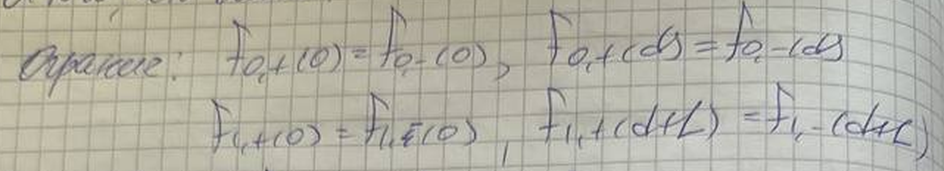
\includegraphics[width=0.8\textwidth]{image-gr-usl-f.png}
%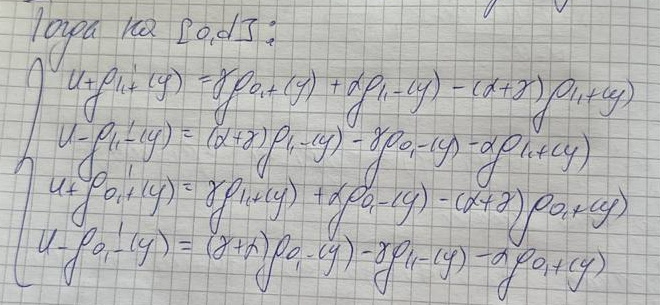
\includegraphics[width=0.8\textwidth]{image-4d-ur.png}
%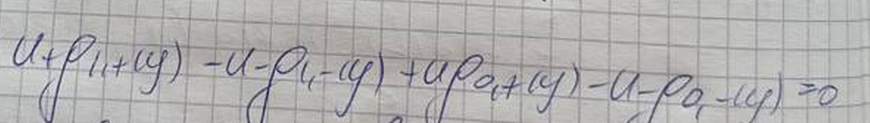
\includegraphics[width=0.8\textwidth]{image-otsyuda.png}

Мы будем искать такую меру $\mu$ на $Z$, что ее ограничения на подмножества $X_{\theta, \pm}$ задавались бы с помощью функции плотности
\begin{equation}\label{density_2}
    g_{\theta, \pm} := \frac{\mu_{\theta, \pm} (dy)}{dy}.
\end{equation}
Для начала представим, что
\begin{equation*}
    \begin{aligned}
        f_{\theta, \pm} (y) &= \displaystyle\int_0^y \psi (x) dx, \qquad y \in [0, d]\\
        f_{1, \pm} (y) &\equiv \displaystyle\int_0^d \psi (x) dx = {const}, \quad y \in (d, d + L],
    \end{aligned}
\end{equation*}
где $\psi (x) \in \mathrm{C}_{0} [0, d]$ и $\psi (0) = f_{\theta, +}' (0) =  \psi (d) = f_{\theta, -}' (d) = 0$. Несложно убедиться, что так определенные функции $f_{\theta, \pm}$ удовлетворяют граничным условиям ~\eqref{restrict_2}. Обратим внимание, что в силу определения $f_{1, \pm}$ на $(d, d + L]$, справедливо $f_{1, \pm}' (y) = 0$ при $y \in (d, d + L]$. Тогда с учетом ~\eqref{density_2} получим, что ~\eqref{main_eq} имеет вид
\begin{equation*}
    \begin{aligned}
    &\int_0^d -u_- \psi (y)  g_{0,-} (y) dy 
    &+ \int_0^d u_+ \psi (y) g_{0,+} (y) dy &+ \\
    + &\int_0^d -u_- \psi (y) g_{1,-} (y) dy
    &+ \int_0^{d} u_+ \psi (y) g_{1,+} (y) dy &= 0.
    \end{aligned}
\end{equation*}
Отсюда, в силу произвольности $\psi (\cdot)$ из класса $\mathrm{C}_0$ и свойств интеграла Лебега, имеем соотношение на плотности
\begin{equation}\label{cond_2}
    u_+ \Bigl(g_{0,+} (y) + g_{1,+} (y) \Bigr) = u_- \Bigl(g_{0,-} (y) + g_{1,-} (y) \Bigr), \quad y \in (0, d).
\end{equation}
Обратим внимание, что если взять $\psi (0) = f_{\theta, +}' (0) = 0, \quad \psi (d) = f_{\theta, -}' (d) = 1$, то, с учетом ~\eqref{cond_2}, получим
$$\mu_{0,-} \{d\} \cdot \left( - u_- f_{0,-}' (d) \right) = 0 \quad \Longrightarrow \quad  \mu_{0,-} \{d\} = 0.$$
С другой стороны, если положить $\psi (0) = f_{\theta, +}' (0) = 1, \quad \psi (d) = f_{\theta, -}' (d) = 0$, то получим связь
\begin{equation*}
    \begin{aligned}
  1 \cdot u_+  \Bigl( \mu_{0,+} \{0\} + \mu_{1,+} \{0\}\Bigr) = 0 \quad &\Longrightarrow \quad \mu_{0,+} \{0\} = - \mu_{1,+} \{0\} \ge 0 \\
  &\Longrightarrow \quad \mu_{0,+} \{0\} = \mu_{1,+} \{0\} = 0.      
    \end{aligned}
\end{equation*}

Итак, допустим теперь, что 
\begin{equation*}
    \begin{aligned}
        f_{\theta, \pm} (y) &\equiv 0, \quad y \in [0, d]\\
        f_{1, +} (y) &\equiv 0, \quad y \in (d, d + L]\\
        f_{1, -} (y) &= f (y), \quad y \in (d, d + L],
    \end{aligned}
\end{equation*}
где $f(y) \in C^{(1)} [d, d + L]$ и $f (d) = 0$. Заметим, что в силу граничных условий ~\eqref{restrict_2}, необходимо требовать $f (d + L) = 0$. Предположим также, что $f' (d + L) = 0$. Тогда ~\eqref{main_eq} примет вид
\begin{equation*}
    \begin{aligned}
        \int_d^{d + L} \Bigl[-u_- f' (y) - f(y) \left(\alpha + \gamma \right) \Bigr] g_{1,-} (y) dy + \int_d^{d + L} \alpha f(y) g_{1,+} (y) dy = 0.
    \end{aligned}
\end{equation*}
Пользуясь формулой интегрирования по частям, а также граничными условиями ~\eqref{restrict_2}, получим
\begin{equation*}
    \begin{aligned}
        -u_- f (y) g_{1,-} (y) \Bigl|_d^{d + L} + \int_d^{d + L} u_- f (y) g_{1,-}' (y) dy &= \int_d^{d + L} u_- f (y) g_{1,-}' (y) dy =\\ 
        = \int_d^{d + L} f(y) \left(\alpha + \gamma \right) g_{1,-} (y) dy &- \int_d^{d + L} \alpha f(y) g_{1,+} (y) dy.
    \end{aligned}
\end{equation*}
Аналогичным образом, в силу произвольности $f (y) \in C^{(1)} [d, d + L]$, имеем
\begin{equation}\label{deriv_1_-}
    g_{1,-}' (y) = \frac{1}{u_-} \Bigl[ \left(\alpha + \gamma \right) g_{1,-} (y) - \alpha g_{1,+} (y)\Bigr], \quad y \in (d, d + L).
\end{equation}
Заметим, что если взять $f' (d + L) = 1$, то, с учетом уже найденного соотношения ~\eqref{deriv_1_-} во внутренних точках $(d, d + L)$, имеет место
$$\mu_{1,-} \{ d + L \} \cdot \left( - u_- f' (d + L) \right)  = 0 \quad \Longrightarrow \quad \mu_{1,-} \{ d + L \} = 0.$$

Итак, мы знаем теперь, что мера граничных точек $0, d$ и $d + L$ равна нулю. Рассмотрим подробнее, какие соотношения на плотности имеют место во внутренних точках. Для этого без ограничения общности рассмотрим следующие функции
\begin{equation*}
    \begin{aligned}
        f_{1, \pm} (y) &\equiv 0, \quad y \in [0, d + L]\\
        f_{0, -} (y) &\equiv 0, \quad y \in [0, d]\\
        f_{0, +} (y) & = f(y) \in C^{(1)} [0, d]
    \end{aligned}
\end{equation*}
Как обычно, из ограничений на границах, будем требовать, чтобы $f (0) = f (d) = 0$. Тогда имеет место
\begin{equation*}
    \begin{aligned}
        \int_0^{d} \alpha f(y) g_{0,-} (y) dy + \int_0^{d} \Bigl[u_+ f' (y) - f(y) \left(\alpha + \gamma \right) \Bigr] g_{0,+} (y) dy + \int_0^{d} \gamma f(y) g_{1,+} (y) dy= 0.
    \end{aligned}
\end{equation*}
Далее, после интегрирования по частям и применения граничных условий, имеем
$$\int_0^{d} f(y) \Bigl[ \alpha g_{0,-} (y) - \left(\alpha + \gamma \right) g_{0,+} (y) + \gamma g_{1,+} (y) \Bigr] dy = \int_0^{d} u_+ f (y) g_{0,+}' (y) dy .$$
Откуда в силу произвольности $f \in C^{(1)} [0, d]$
$$g_{0,+}' (y) = \frac{1}{u_+} \Bigl[ \alpha g_{0,-} (y) - \left(\alpha + \gamma \right) g_{0,+} (y) + \gamma g_{1,+} (y) \Bigr], \quad y \in (0, d).$$
Положив нулем $f_{0, +} (y) = 0$ на $[0, d]$ и взяв за $f (y)$ поочередно оставшиеся функции, получим целую систему дифференциальных уравнений
\begin{equation*}
\left\{ \begin{aligned} 
g_{1, +}'(y) &= \frac{1}{u_+} \Bigl[ \gamma g_{0, +}(y) + \alpha g_{1, -}(y) -(\alpha + \gamma) g_{1, +}(y)&\Bigr]\\
g_{1, -}'(y) &= \frac{1}{u_-} \Bigl[ -\gamma g_{0, -}(y) - \alpha g_{1, +}(y) + (\alpha + \gamma) g_{1, -}(y)&\Bigr]\\
g_{0, +}'(y) &= \frac{1}{u_+} \Bigl[ \gamma g_{1, +}(y) + \alpha g_{0, -}(y) - (\alpha + \gamma) g_{0, +}(y)&\Bigr]\\
g_{0, -}'(y) &= \frac{1}{u_-} \Bigl[ -\gamma g_{1, -}(y) - \alpha g_{0, +}(y) + (\alpha + \gamma) g_{0, -}(y)&\Bigr]
\end{aligned}
\right., \quad y \in (0, d)
\end{equation*}

Далее, подобно тому, как мы получили соотношение ~\eqref{deriv_1_-}, при следующей подстановке функций
\begin{equation*}
    \begin{aligned}
        f_{\theta, \pm} (y) &\equiv 0, \quad y \in [0, d]\\
        f_{1, -} (y) &\equiv 0, \quad y \in (d, d + L]\\
        f_{1, +} (y) &= f (y), \quad y \in (d, d + L],
    \end{aligned}
\end{equation*}
наконец, получим
$$g_{1, +}'(y) = \frac{1}{u_+} \Bigl[ \alpha g_{1, -}(y) -(\alpha + \gamma) g_{1, +}(y)\Bigr], \quad y \in (d, d + L).$$
И на этом мы завершаем доказательство теоремы.
\begin{flushright}
$\blacksquare$
\end{flushright}
\begin{zam}
При $\gamma = 0$, то есть когда возмущения верхней границы нет, системы дифференциальных уравнений ~\eqref{syst_4} и ~\eqref{syst_2} в совокупности распадаются на две независимые подсистемы. А именно, на 
\begin{equation*}
\left\{ \begin{aligned} 
g_{0, +}'(y) &= \frac{\alpha}{u_+} \Bigl[ g_{0, -}(y) - g_{0, +}(y)\Bigr]\\
g_{0, -}'(y) &= \frac{\alpha}{u_-} \Bigl[ g_{0, -}(y) - g_{0, +}(y)\Bigr]
\end{aligned}
\right., \qquad y \in (0, d)
\end{equation*}
и
\begin{equation*}
\left\{ \begin{aligned} 
g_{1, +}'(y) &= \frac{\alpha}{u_+} \Bigl[ g_{1, -}(y) - g_{1, +}(y)\Bigr]\\
g_{1, -}'(y) &= \frac{\alpha}{u_-} \Bigl[ g_{1, -}(y)- g_{1, +}(y) \Bigr]
\end{aligned}
\right., \qquad y \in (0, d + L)
\end{equation*}
Как и следовало ожидать, эти две системы аналогичны тем, что мы видели в исходной упрощенной модели ~\eqref{simple_case}.
\end{zam}

\section{Заключение}

Итак, нами были рассмотрены две стохастические модели, описывающие движение частиц на вещественной прямой, а также получены результаты по описанию стационарного распределения в этих процессах. Найденные результаты для модели с возмущением верхней границы позволяют приступить к поиску плотности в явном виде. Более того, в дальнейшем все описанные результаты можно расширить на составные модели. А именно, на модели предполагающие несколько лидеров и участников.

\newpage
\nocite{*}
\bibliographystyle{abbrv}
\bibliography{diploma}
\begin{thebibliography}{9}
%\bibliographystyle{acm}

\bibitem{Venz} А. Д. Вентцель (1975).
\newblock Курс теории случайных процессов. 
\newblock Главная редакция физико-математической литературы изд-ва ``Наука''.

\bibitem{Bulin} А. В. Булинский, А. Н. Ширяев (2005).
\newblock Теория случайных процессов. 
\newblock ФИЗМАТЛИТ.

\end{thebibliography}
\end{document}
Итак, с учетом заданных граничных условий, а именно
\begin{equation*}
\left\{ \begin{aligned} 
f_{0, +}(0) &= f_{0, -}(0), \quad f_{0, +}(d) = f_{0, -}(d)\\
f_{1, +}(0) &= f_{1, -}(0), \quad f_{1, +}(d + L) = f_{1, -}(d + L)
\end{aligned}
\right.
\end{equation*}
имеем две системы дифференциальных уравнений. \\
Одну, определенную на $[0, d]$:
\begin{equation}\label{5}
\left\{ \begin{aligned} 
g_{1, +}'(y) &= \frac{1}{u_+} \Bigl[ \gamma g_{0, +}(y) + \alpha g_{1, -}(y) -(\alpha + \gamma) g_{1, +}(y)\Bigr]\\
g_{1, -}'(y) &= \frac{1}{u_-} \Bigl[ -\gamma g_{0, -}(y) - \alpha g_{1, +}(y) + (\alpha + \gamma) g_{1, -}(y)\Bigr]\\
g_{0, +}'(y) &= \frac{1}{u_+} \Bigl[ \gamma g_{1, +}(y) + \alpha g_{0, -}(y) - (\alpha + \gamma) g_{0, +}(y)\Bigr]\\
g_{0, -}'(y) &= \frac{1}{u_-} \Bigl[ -\gamma g_{1, -}(y) - \alpha g_{0, +}(y) + (\alpha + \gamma) g_{0, -}(y)\Bigr]
\end{aligned}
\right.
\end{equation}
и вторую на $(d, d + L]$:
\begin{equation*}
\left\{ \begin{aligned} 
g_{1, +}'(y) &= \frac{1}{u_+} \Bigl[ \alpha g_{1, -}(y) -(\alpha + \gamma) g_{1, +}(y)\Bigr]\\
g_{1, -}'(y) &= \frac{1}{u_-} \Bigl[- \alpha g_{1, +}(y) + (\alpha + \gamma) g_{1, -}(y) \Bigr]
\end{aligned}
\right.
\end{equation*}

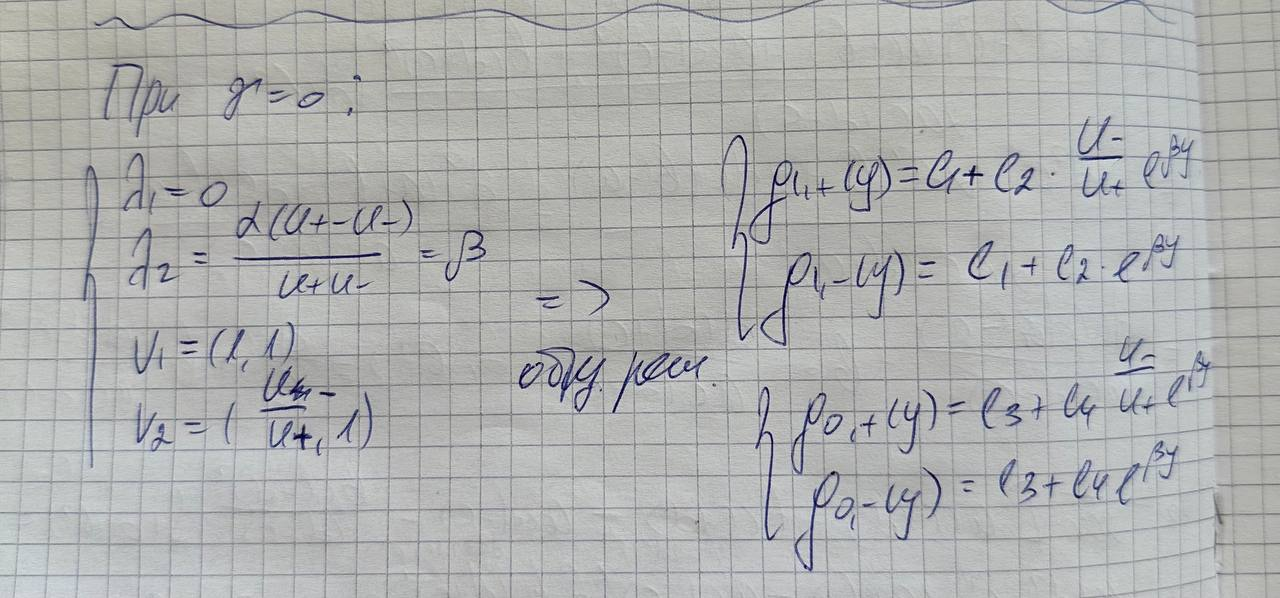
\includegraphics[width=0.8\textwidth]{solution_gamma_0.png}

Но вернемся к возмущенной системе. Обозначим собственные числа системы, как $\{ \lambda_i\}_{i=1}^4$, а собственные вектора $\{ v_i\}_{i=1}^4$ и его коодинаты $v_i^j, j = 1, ..., 4$. Тогда общее решение системы \ref{5} можно записать в виде
\begin{equation*}
\left\{ \begin{aligned} 
g_{1, +}(y) = c_1 v_1^1 e^{\lambda_1 y} + c_2 v_2^1 e^{\lambda_2 y} + c_3 v_3^1 e^{\lambda_3 y} + c_4 v_4^1 e^{\lambda_4 y}\\
g_{1, -}(y) = c_1 v_1^2 e^{\lambda_1 y} + c_2 v_2^2 e^{\lambda_2 y} + c_3 v_3^2 e^{\lambda_3 y} + c_4 v_4^2 e^{\lambda_4 y}\\
g_{0, +}(y) = c_1 v_1^3 e^{\lambda_1 y} + c_2 v_2^3 e^{\lambda_2 y} + c_3 v_3^3 e^{\lambda_3 y} + c_4 v_4^3 e^{\lambda_4 y}\\
g_{0, -}(y) = c_1 v_1^4 e^{\lambda_1 y} + c_2 v_2^4 e^{\lambda_2 y} + c_3 v_3^4 e^{\lambda_3 y} + c_4 v_4^4 e^{\lambda_4 y}
\end{aligned}
\right.
\end{equation*}

Распишем собственные значения при малых $\gamma$. Имеем

\begin{equation*}
\begin{aligned} 
\lambda_1 &= 0\\
\lambda_2 &= \frac{\alpha (u_+ - u_-)}{u_+ u_-} = \beta\\
\lambda_3 &= \frac{\alpha (u_+ - u_-)}{u_+ u_-} - \gamma \frac{2(u_+^2 + u_-^2)}{(u_- - u_+) u_+ u_-} + o(\gamma^2) \\
\lambda_4 &= 0 + \gamma \frac{4}{(u_- - u_+)} + o(\gamma^2)
\end{aligned}
\end{equation*}

Аналогично для собственных векторов
\begin{equation*}
\begin{aligned} 
v_1 &= \Bigl( 1, 1, 1, 1\Bigr)^\intercal\\
v_2 &= \Bigl( 1, \frac{u_+}{u_-}, 1, \frac{u_+}{u_-}\Bigr)^\intercal\\
v_3^1 &= \alpha u_- (u_+^2 + u_-^2) + \gamma \cdot 2 u_-^2 \frac{(u_+^2 + u_+ u_- + 2 u_-^2)}{(u_- - u_+)} + o(\gamma^2) \\
v_3^3 &= -  \alpha u_- (u_+^2 + u_-^2) - \gamma \cdot 2 u_-^2 \frac{(u_+^2 + u_+ u_- + 2 u_-^2)}{(u_- - u_+)} + o(\gamma^2) \\
v_3^2 &= \alpha u_+ (u_+^2 + u_-^2) + \gamma \cdot 2 u_+ \Bigl( u_+^2 + u_-^2 + u_+ u_-\Bigr) + o(\gamma^2) \\
v_3^4 &= - \alpha u_+ (u_+^2 + u_-^2) - \gamma \cdot 2 u_+  \Bigl( u_+^2 + u_-^2 + u_+ u_-\Bigr) + o(\gamma^2) \\
v_4^1 &= \alpha - \gamma \cdot \frac{(3 u_- + u_+)}{(u_- - u_+)} + o(\gamma^2) \\
v_4^3 &= - \alpha + \gamma \cdot \frac{(3 u_- + u_+)}{(u_- - u_+)} + o(\gamma^2) \\
v_4^2 &= \alpha - \gamma + o(\gamma^2)\\
v_4^4 &= - \alpha + \gamma+ o(\gamma^2)
\end{aligned}
\end{equation*}

Заметим, что при $\alpha = 0$ и $\gamma > 0$ общее решение системы на $[0, d]$ будет иметь вид
\begin{equation*}
\left\{ \begin{aligned} 
g_{1, +}(y) &= c_1 + c_2 + c_3 \cdot \gamma \cdot 2 u_-^2 \frac{(u_+^2 + u_+ u_- + 2 u_-^2)}{(u_- - u_+)} e^{- \gamma \frac{2(u_+^2 + u_-^2)}{(u_- - u_+) u_+ u_-} y} - c_4 \cdot \gamma \cdot \frac{(3 u_- + u_+)}{(u_- - u_+)} e^{\gamma \frac{4}{(u_- - u_+)} y}\\
g_{1, -}(y) &= c_1 + c_2 \cdot \frac{u_+}{u_-} + c_3 \cdot \gamma \cdot 2 u_+ \Bigl( u_+^2 + u_-^2 + u_+ u_-\Bigr) e^{- \gamma \frac{2(u_+^2 + u_-^2)}{(u_- - u_+) u_+ u_-} y} - c_4 \cdot \gamma e^{\gamma \frac{4}{(u_- - u_+)} y}\\
g_{0, +}(y) &= c_1 + c_2 - c_3 \cdot \gamma \cdot 2 u_-^2 \frac{(u_+^2 + u_+ u_- + 2 u_-^2)}{(u_- - u_+)} e^{- \gamma \frac{2(u_+^2 + u_-^2)}{(u_- - u_+) u_+ u_-} y} + c_4 \cdot \gamma \cdot \frac{(3 u_- + u_+)}{(u_- - u_+)} e^{\gamma \frac{4}{(u_- - u_+)} y}\\
g_{0, -}(y) &= c_1 + c_2 \cdot \frac{u_+}{u_-} - c_3 \cdot \gamma \cdot 2 u_+ \Bigl( u_+^2 + u_-^2 + u_+ u_-\Bigr) e^{- \gamma \frac{2(u_+^2 + u_-^2)}{(u_- - u_+) u_+ u_-} y} + c_4 \cdot \gamma e^{\gamma \frac{4}{(u_- - u_+)} y} 
\end{aligned}
\right.
\end{equation*}
Сопоставим с системой, полученной зануелнием $\alpha$.

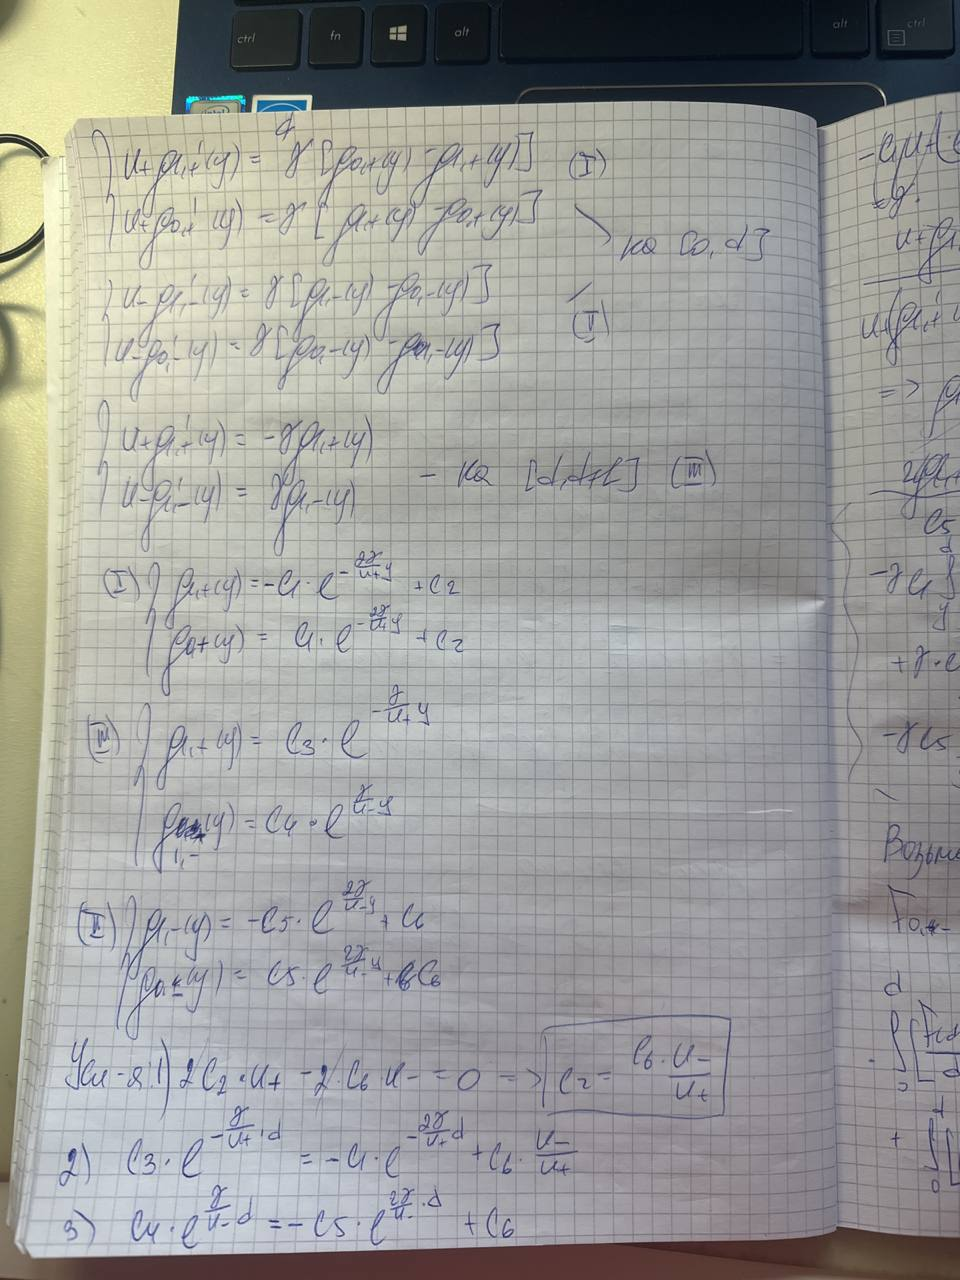
\includegraphics[width=0.8\textwidth]{system_alpha_0.jpg}

2) Рассмотрим систему дифференциальных уравнений на $(d, d + L]$.
\begin{equation*}
\left\{ \begin{aligned} 
g_{1, +}'(y) &= \frac{1}{u_+} \Bigl[ \alpha g_{1, -}(y) -(\alpha + \gamma) g_{1, +}(y)\Bigr]\\
g_{1, -}'(y) &= \frac{1}{u_-} \Bigl[- \alpha g_{1, +}(y) + (\alpha + \gamma) g_{1, -}(y) \Bigr]
\end{aligned}
\right.
\end{equation*}
с собственнымми значениями и векторами, удовлетворяющим

\begin{equation*}
\begin{aligned} 
\lambda_1 &= \frac{\alpha (u_+ - u_-)}{u_+ u_-} - \gamma \frac{(u_+^2 + u_-^2)}{(u_- - u_+) u_+ u_-} + o(\gamma^2) \\
\lambda_2 &= 0 + \gamma \frac{2}{(u_- - u_+)} + o(\gamma^2)\\
v_1^1 &= \frac{u_-}{u_+} + \gamma \frac{u_- (u_+ + u_-)}{\alpha u_+ (u_- - u_+)} + o(\gamma^2) \\
v_2^1 &= 1 - \gamma \frac{(u_+ + u_-)}{\alpha (u_- - u_+)} + o(\gamma^2) \\
v_1^2 &= v_2^2 = 1 \\
\end{aligned}
\end{equation*}
При $\gamma = 0$ общее решение системы имеет вид
\begin{equation*}
\left\{ \begin{aligned} 
g_{1, +}(y) &= c_1 \frac{u_-}{u_+} e^{\beta y} + c_2\\
g_{1, -}(y) &= c_1 e^{\beta y} + c_2
\end{aligned}
\right.
\end{equation*}
При малых $\gamma$ решение на $(d, d + L]$ задается как
\begin{equation*}
\left\{ \begin{aligned} 
g_{1, +}(y) &= c_1 \Bigl(\frac{u_-}{u_+} + \gamma \frac{u_- (u_+ + u_-)}{\alpha u_+ (u_- - u_+)}\Bigr) e^{\beta y - \gamma \frac{(u_+^2 + u_-^2)}{(u_- - u_+) u_+ u_-} y} + c_2 \Bigl( 1 - \gamma \frac{(u_+ + u_-)}{\alpha (u_- - u_+)}\Bigr) e^{\gamma \frac{2}{(u_- - u_+)} y}\\
g_{1, -}(y) &= c_1 e^{\beta y - \gamma \frac{(u_+^2 + u_-^2)}{(u_- - u_+) u_+ u_-} y} + c_2 e^{\gamma \frac{2}{(u_- - u_+)} y}
\end{aligned}
\right.
\end{equation*}




\begin{figure}[h]
  \centering
  \begin{tikzpicture}
    \begin{axis}[
        xmin=-1, xmax=3,
        ymin=-1, ymax=3,
        axis lines=middle,
      ]  
      \addplot[samples=100, domain=0:3, name path=A] {3/(2*x+1)}; 
      \addplot[samples=50, domain=0:3,name path=B] {3*x-2}; 
      \path[name path=xaxis] (\pgfkeysvalueof{/pgfplots/xmin}, 0) -- (\pgfkeysvalueof{/pgfplots/xmax},0);
       \addplot[gray, pattern=north west lines] fill between[of=B and xaxis, soft clip={domain=0.66666:1}];
      \addplot[gray, pattern=north west lines] fill between[of=A and xaxis, soft clip={domain=1:2}];
      \addplot +[mark=none] coordinates {(2, -1) (2, 3)};
    \end{axis}
  \end{tikzpicture}
\end{figure}